\apendice{Pruebas de rendimiento de componentes}


Teniendo en cuenta los requisitos descritos en el anexo anterior, se realiza una comparación para elegir el sistema 
gestor de bases de datos y el modelo de predicción que mejor cumplan dichos requisitos.

\section{Estudio del sistema gestor de bases de datos}

\subsection{Metodología de la comparación}

\subsubsection{Sistemas de gestión de bases de datos bajo estudio}

Lo primero a tener en cuenta es el modelo de la base de datos que se va a utilizar, ya que tendrá una gran importancia
a la hora de decidir qué sistema de gestión de bases de datos se va a utilizar. Los siguientes modelos \cite{10.5555/3364297} han sido
tenidos en cuenta:

\begin{itemize}
    \item Bases de datos relacionales: en estos sistemas, la información se almacena en relaciones. Una relación,
        definidas también como tablas, es una colección de tuplas, o filas. Las relaciones se definen por su nombre
        y un número fijo de atributos, o columnas, con tipos de datos fijos. Estos sistemas respetan las propiedades
        ACID (Atomicity, Consistency, Isolation y Durability), y tienen operaciones básicas definidas, como la selección,
        proyección y unión.
    \item Bases de datos de documentos: la principal característica de estas bases de datos es la organización de los datos
        de forma libre, sin seguir ningún esquema. Esto significa, por contrario que en las bases de datos relacionales,
        las entradas no poseen una estructura uniforme, las columnas pueden tener más de un valor e incluso pueden almacenar
        estructuras anidadas.
    \item Bases de datos de Clave-valor: son las bases de datos más simples y solo almacenan pares clave-valor. Normalmente
        no son factibles para aplicaciones complejas, pero normalmente presentan un gran rendimiento debido a su
        simplicidad.
    \item Motores de búsqueda: su uso principal es la búsqueda de datos, y son típicamente NoSQL, es decir, que no siguen
        un modelo relacional.
    \item Bases de datos de series temporales: estas bases de datos están optimizadas para almacenar series temporales \cite{influx:timeseries}.
        Aunque son típicamente NoSQL, bases de datos de series temporales relacionales existen.
\end{itemize}

Cualquiera de estos modelos permiten el manejo de información de series temporales, como la información que recibimos
de los AGV. Sin embargo, las bases de datos de series temporales están especializadas en este tipo de trabajos, por lo que
las hace perfectas para nuestras necesidades.

Como selección inicial, se han escogido los cinco sistemas gestores de bases de datos de series temporales más temporales
según el ranking DB-Engines \cite{dbengines:rankingTSDBMS}. Este ranking es utilizado en otros estudios, como \cite{10.1007/978-3-030-50426-7_28}.
Los sistemas gestores de bases de datos elegidos para comparar son:

\begin{itemize}
    \item \textbf{InfluxDB 2.6.1} Un sistema gestor de bases de datos de series temporales desarrollado por InfluxData. Su
        uso principal es el almacenamiento y obtención de series temporales, creadas en operaciones de monitoreo de IoT,
        información de sensores, etc.
    \item \textbf{kdb+ 4.0} Una base de datos de series temporales relacional desarrollado por KX, usado principalmente en
        negociación bursátil de alta frecuencia, para almacenar y para procesar datos a una alta velocidad.
    \item \textbf{Prometheus 2.43.0} Una base de datos de series temporales usada para el monitoreo de eventos y alarmas, que
        utiliza un modelo HTTP.
    \item \textbf{Graphite 1.1.10} Una herramienta que almacena, monitoriza y grafica series temporales numéricas.   
    \item \textbf{TimescaleDB 2.10.1} Una base de datos de código abierto, desarrollada como complemento a PostgreSQL con el
        fin de mejorar el rendimiento y análisis para series temporales.
\end{itemize}

Aunque este ranking solo mide la popularidad y ordena los sistemas en función de atributos sociales, es especialmente
útil para soluciones de código abierto, pues esto generalmente significa que está soportada por una comunidad activa
con muchos colaboradores involucrados en añadir nueva funcionalidad y corregir errores.

\subsubsection{Procedimiento de la comparación}
La comparación y el filtrado de los modelos seleccionados ha sido realizados en tres pasos secuenciales:
\begin{enumerate}
    \item Información general, soporte software y apoyo de la comunidad.
    \item Modelo de datos y especificaciones técnicas.
    \item Prueba de rendimiento.
\end{enumerate}

En los primeros dos pasos, los sistemas comparados que no cumplan los requisitos especificados en secciones anteriores
han sido descartados. Después, con los sistemas restantes, se ha realizado una prueba de rendimiento con el fin de
tomar la decisión final. A su vez, esta prueba se divide en otras dos pruebas.

\imagen{DiagramaTests1}{Procedimiento de la prueba de inserción}
\imagen{DiagramaTests2}{Procedimiento de la prueba de latencia}

El primer test, (Figura \ref{fig:DiagramaTests1}) mide el uso de CPU y RAM del sistema cuando se insertan datos de forma
masiva, así como el tiempo tomado y el número de inserciones por segundo realizadas. En total, 300.000 entradas son enviadas,
formadas por los siguientes campos: timestamp, id del vehículo, batería, velocidad, posición en la coordenada x, posición
en la coordenada y, temperatura y voltaje. Para realizar la prueba de manera más realista, los datos se insertan en la
base de datos en tandas de 5.000. Para ello se almacenan primero en un buffer controlado por el servicio ``Receiver'', ya
que de esta manera se obtiene un mejor rendimiento que si se insertasen de uno en uno. Para medir el uso de CPU y de RAM
de la misma forma con todos los diferentes gestores, las medidas son tomadas de lo que reporta el estado del contenedor
de Docker en el que se ejecutan dichos sistemas.

En el segundo test (Figura \ref{fig:DiagramaTests2}) se mide la latencia de inserción. Esto es, el tiempo que tarda
en estar disponible una entrada después de su inserción. Para esto, un script de Python, formado por dos hilos, ha sido creado.
El primero de esos hilos realiza la inserción en la base de datos y el otro intenta obtener dicha entrada en un bucle.
En el momento en el que dicha entrada se obtiene, se anota dicho tiempo y se resta del momento en le que se insertó
la entrada. Este test se realiza 200 veces y se hace una media con los resultados.

Cada test se realiza cinco veces para reducir la variabilidad, tomando la media de dichas ejecuciones como valor final.

\subsubsection{Métricas de la comparación} 
A continuación se detallan las métricas utilizadas para realizar la comparación.

% \textbf{Información general, soporte de software y comunidad}

Las métricas de información general analizan:
\begin{itemize}
    \item Organización: que organización o compañía es responsable del desarrollo y mantenimiento del sistema.
    \item Año de lanzamiento: en que año se lanzó inicialmente.
    \item Última versión: en que año se lanzó la última versión.
    \item Licencia: que tipo de licencia tiene el software: código abierto (OSS), o licencia comercial.
\end{itemize}
El indicador de rendimiento del soporte de software analiza:
\begin{itemize}
    \item Sistema Operativo: qué sistemas operativos se soportan.
    \item Soporte para Python: como el sistema está implementado en Python, nos interesa que el sistema tenga
        buen soporte de este lenguaje.
    \item Lenguaje de consultas: que lenguaje de consultas soporta el sistema.
    \item Plugins para aprendizaje automático: si el sistema soporta complementos que simplifiquen la predicción de nuevos
        datos.
\end{itemize}
La comparación del soporte de la comunidad contiene:
\begin{itemize}
    \item Número de estrellas del repositorio de GitHub: como forma de medir su popularidad.
    \item Pull requests: número de pull requests enviadas en el último mes.
    \item Pull requests aceptadas: número de pull requests aceptadas en el último mes.
    \item Issues: número de issues creados en el último mes.
    \item Issues cerrados: número de issues cerrados en el último mes.
\end{itemize}
Estos cuatro últimos campos se usarán para comparar que comunidad es más activa.

% \textbf{Modelo de datos e información técnica}

El indicador de rendimiento del modelo de datos compara:
\begin{itemize}
    \item Modelo de datos: que modelo concreto implementa cada sistema.
    \item Esquema: un esquema puede verse como una plantilla que define como se almacena la información. Este campo
        compara si la organización de los datos es estricta (esquema fijo) o no (esquema libre).
    \item Índices secundarios: si el sistema soporta índices secundarios para un mejor rendimiento de consultas o no.
    \item Precisión temporal: unidad mínima de tiempo que puede tener una entrada.
\end{itemize}

El indicador de rendimiento de información técnica se compone de los siguientes campos:
\begin{itemize}
    \item Scripts de servidor: si el sistema es capaz de ejecutar scripts en el servidor o no.
    \item Método de partición: si se soportan o no métodos de partición para una mayor escalabilidad.
    \item Replicación: que métodos de replicación soporta.
    \item Consistencia: si la información escrita es consistente o no.
    \item Conformidad con ACID: si el sistema sigue los principios ACID o no.
    \item Concurrencia: si el sistema soporta accesos concurrentes o no.
    \item Durabilidad: si la información es persistente, incluso si falla.
    \item Método de inserción: si la información se introduce mediante una consulta de inserción o extrayendo los
        datos de un endpoint de forma periódica.
\end{itemize}

% \textbf{Análisis de rendimiento}

Por último, el análisis de rendimiento compara:
\begin{itemize}
    \item Tiempo de inserción: tiempo que se tarda en hacer la prueba de inserción en segundos.
    \item Tasa de transferencia: número de inserciones por segundo.
    \item Uso de la CPU: uso de la CPU del contenedor de Docker en el que se ejecuta base de datos durante 
        la primera prueba.
    \item Uso de RAM: uso de RAM del contenedor de Docker en el que se ejecuta la base de datos durante la
        primera prueba.
    \item Latencia: tiempo que tarda en ejecutarse la segunda prueba en milisegundos.
\end{itemize}

\subsection{Experimentos y resultados}

\begin{table}[H]
    \begin{center}
        \begin{adjustbox}{max width=\textwidth}
            \rowcolors{2}{gray!35}{}
            \begin{tabular}{l c c c c}
                \toprule
                Sistema & Organización & Lanzamiento & Última versión & Licencia \\
                \otoprule
                InfluxDB    & InfluxData & 2013 & 2023 & MIT \\
                kdb+        & Kx Systems & 2000 & 2020 & Comercial \\
                Prometheus  & -          & 2015 & 2023 & Apache License 2.0 \\
                Graphite    & -          & 2006 & 2022 & Apache License 2.0 \\
                TimescaleDB & Timescale  & 2017 & 2023 & Apache License 2.0 \\
                \bottomrule
            \end{tabular}
        \end{adjustbox}
        \caption{Comparativa de información general}
        \label{tabla:gisgbd}
    \end{center}
\end{table}

\subsubsection{Información general (Tabla \ref{tabla:gisgbd})} Solo software de código abierto será considerado en este
trabajo. Aunque kdb+ tiene una versión de 32 bits, no se usará y no volverá a aparecer en las siguientes comparaciones.
Por esta razón también, solo las características de la ``Comunity Edition'' de InfluxDB serán utilizadas en dichas
comparaciones, y características de la ``Enterprise Edition'', que no es de código abierto, no se tendrán en cuenta.

\begin{table}[H]
    \begin{center}
        \begin{adjustbox}{max width=\textwidth}
            \begin{tabular}{l c c c c}
                \toprule
                Sistema & OS & Python & Lenguaje de consultas & Plugins ML\\
                \otoprule
                & Linux &                       &  \\
                \multirow{-2}{*}{InfluxDB} & OS x  & \multirow{-2}{*}{Sí} & \multirow{-2}{*}{Flux e InfluxQL} & \multirow{-2}{*}{Loud ML} \\
                \rowcolor{gray!35}
                                            & Linux   &                        & & \\
                \rowcolor{gray!35}
                \multirow{-2}{*}{Prometheus} & Windows & \multirow{-2}{*}{Sí}  & \multirow{-2}{*}{PromQL} & \multirow{-2}{*}{No}\\
                                        & Linux &                       &  & \\
                \multirow{-2}{*}{Graphite} & Unix  & \multirow{-2}{*}{Sí}  & \multirow{-2}{*}{No} & \multirow{-2}{*}{No} \\
                \rowcolor{gray!35}
                                            & Linux   &                             & & \\
                \rowcolor{gray!35}
                                            & OS X    &                             & & \\
                \rowcolor{gray!35}
                \multirow{-3}{*}{TimescaleDB} & Windows & \multirow{-3}{*}{Sí} & \multirow{-3}{*}{SQL} & \multirow{-3}{*}{No} \\
                \bottomrule
            \end{tabular}
        \end{adjustbox}
        \caption{Soporte software}
        \label{tabla:sssgbd}
    \end{center}
\end{table}

\subsubsection{Soporte software (Tabla \ref{tabla:sssgbd})} Todos los sistemas soportan Linux y Python, el sistema operativo 
y lenguaje utilizados. Solo Graphite no tiene un lenguaje de consultas definido, aunque se pueden realizar utilizando lo que 
llaman Funciones \cite{graphite-functions}. Únicamente InfluxDB soporta complementos para aprendizaje automático. Otros sistemas como
TimescaleDB proveen documentación para realizarlo de forma externa en lenguajes como Python o R \cite{timescale-forecasting}.

\begin{table}[H]
    \begin{center}
        \begin{adjustbox}{max width=\textwidth}
            \rowcolors{2}{gray!35}{}
            \begin{tabular}{l c c c c c c}
                \toprule
                \multirow{2}{*}{Sistema} & Estrellas & \multirow{2}{*}{Pull requests} & Pull requests & \multirow{2}{*}{Issues}  & Issues \\
                 &  GitHub &  & aceptadas &  &  cerrados \\
                \otoprule
                InfluxDB    & 25.2k & 26 & 22 & 37 & 13 \\
                Prometheus  & 47.4k & 75 & 53 & 42 & 20\\
                Graphite & 5.6k & 0 & 0 & 0 & 0 \\
                TimescaleDB & 14.7k & 105 & 83 & 67 & 46 \\
                \bottomrule
            \end{tabular}
        \end{adjustbox}
        \caption{Soporte de la comunidad}
        \label{tabla:cssgbd}
    \end{center}
\end{table}

\subsubsection{Soporte de la comunidad (Tabla \ref{tabla:cssgbd})} Como muestra la tabla, todos los proyectos son muy
activos a excepción de Graphite.

\begin{table}[H]
    \begin{center}
        \begin{adjustbox}{max width=\textwidth}
            \begin{tabular}{l c c c c c}
                \toprule
                \multirow{2}{*}{Sistema} & \multirow{2}{*}{Modelo} & \multirow{2}{*}{Esquema} & \multirow{2}{*}{Tipado} & Índice & Precisión\\
                &&&& secundario & temporal \\
                \otoprule
                &&& Numéricos && \\
                \multirow{-2}{*}{InfluxDB}    & \multirow{-2}{*}{Multidimensional} & \multirow{-2}{*}{Libre} & y strings & \multirow{-2}{*}{No} & \multirow{-2}{*}{Nanosegundos} \\
                \rowcolor{gray!35}
                Prometheus  & Multidimensional & Sí & Numéricos & No & Milisegundos \\
                Graphite    & Key-Value & Sí & Numéricos & No & Segundos \\
                \rowcolor{gray!35}
                TimescaleDB & Relacional & Sí & Tipos SQL & Sí & Nanosegundos \\
                \bottomrule
            \end{tabular}
        \end{adjustbox}
        \caption{Comparativa del modelo de datos}
        \label{tabla:dmsgbd}
    \end{center}
\end{table}

\subsubsection{Comparación del modelo de datos (Tabla \ref{tabla:dmsgbd})} Tanto InfluxDB como Prometheus utilizan un modelo 
multidimensional. Este modelo puede verse como un modelo clave-valor multidimensional: las entradas de datos están formados 
por un campo que describe la información almacenada (``nombre de la métrica'' para Prometheus y ``medida'' para InfluxDB) 
y un set de pares clave-valor asociados con un timestamp. La principal diferencia es que las entradas en el modelo de InfluxDB 
están formados por la medida, un set de etiquetas y un set de valores, en vez de solo un set de pares clave-valor. 
Estas etiquetas guardan metadatos en forma de cadenas de caracteres, son opcionales y están indexados, mientras que el set de 
valores guardan la información, no están indexados y están asociados con un timestamp.

Graphite agrega los datos de manera automática en ventanas de un segundo o más. Este comportamiento no es el deseado 
para nuestras necesidades, ya que se requiere almacenar todos los datos enviados.

\begin{table}[]
    \begin{center}
        \begin{adjustbox}{max width=\textwidth}
            \begin{tabular}{l c c c c}
                \toprule
                Sistema & InfluxDB & Prometheus & Graphite & TimescaleDB \\
                \otoprule
                Scripts del servidor & No & No & No & Sí \\
                \rowcolor{gray!35}
                Particionamiento & No & Sharding & No & Sí \\
                Replicación & No & Sí & No & Sí \\
                \rowcolor{gray!35}
                Consistencia & Eventual & No & No & Inmediata \\
                ACID& No & No & No & Sí \\
                \rowcolor{gray!35}
                Concurrencia & Sí & Sí & Sí & Sí \\
                Durabilidad & Sí & Sí & Sí & Sí \\
                \rowcolor{gray!35}
                Permisos                   & Permisos vía    &                      &                      & Derechos \\
                \rowcolor{gray!35}
                de usuario & cuentas & \multirow{-2}{*}{No} & \multirow{-2}{*}{No} & estándar SQL \\
                Método inserción & Push & Pull & Push & Push \\
                \bottomrule
            \end{tabular}
        \end{adjustbox}
        \caption{Comparativa de información técnica}
        \label{tabla:tisgbd}
    \end{center}
\end{table}

\subsubsection{Comparativa información técnica (Tabla \ref{tabla:tisgbd})} En InfluxDB, la consistencia es eventual. Según
la documentación, se prioriza el rendimiento de lectura y escritura antes que una fuerte consistencia. Se asegura, sin 
embargo, que la información es eventualmente consistente \cite{influx:consistency}.

En bases de datos típicas, la información se inserta a través de algún tipo de consulta desde fuera. Por otro lado, 
Prometheus escucha a un endpoint en el que se publican los datos y se obtienen en intervalos fijos de tiempo. Esto 
significa que la inserción solo ocurrirá cuando Prometheus escuche a dicho endpoint, por lo que la información no se 
puede insertar en cualquier momento. Un método más típico existe, pero no es recomendado y no es posible especificar 
timestamps \cite{prom:pushgateway}.

Solo InfluxDB y TimescaleDB cumplen todos los requisitos, ya que Graphite agrega los datos en ventanas de 1 segundo,
haciendo imposible obtener datos de un momento concreto, y la forma de inserción de Prometheus le hace incompatible 
con nuestras necesidades, ya que es necesario poder insertar datos en cualquier momento. Por esto, solo estos dos
sistemas se compararán en la prueba de rendimiento.

\subsubsection{Análisis del rendimiento} La prueba se realizó con un procesador AMD Ryzen 5 3600 y 32 GB de RAM. Ya que 
este modelo de CPU tiene 12 hilos, el uso de la CPU puede ser tan alto como 1200\% (Uso CPU = Hilos * 100). Los resultados
de esta prueba se muestran en la tabla \ref{tabla:ptsgbd}.

\tablaSmall{Resultados de la prueba de rendimiento}{l c c}{ptsgbd}{
System & InfluxDB & TimescaleDB \\
}{
    Tiempo inserción (s) & 24.13 & \textbf{1.16} \\
    Tasa inserción (I/s) & 12432.66 & \textbf{258620.69} \\
    Uso CPU (\%) & \textbf{15.05} & 55.32 \\
    Uso RAM (MB) & \textbf{219.85} & 373.73 \\
    Latencia (ms) & 3.37 & \textbf{0.22} \\
}

Como se puede observar, InfluxDB es más lento en todos las pruebas que TimescaleDB, pero este último utiliza más 
recursos del sistema. Si en un futuro es necesario escalar InfluxDB puede ser mejor opción, ya que un menor uso de 
recursos suele significar un menor coste. Sin embargo, TimescaleDB es más flexible, ya que al estar basado en PostgreSQL 
tiene todas sus características. Cualquiera de estos dos sistemas puede ser perfectamente usado según los requisitos marcados.

\subsection{Elección final}

Al final, el sistema gestor de bases de datos escogido ha sido InfluxDB. Aunque sea más lento que TimescaleDB, tiene
una velocidad lo suficientemente buena, y al consumir menos recursos la hace una opción más barata en caso de que 
esta solución se aplique comercialmente.

Otro motivo de peso para elegir InfluxDB es que viene por defecto con una interfaz web llamada Chronograf 
(Figura \ref{fig:interfaz}) en la que se puede manejar la base de datos, crear gráficas, establecer alarmas, etc. 
Para realizar esto mismo con TimescaleDB, es necesario utilizar otra herramienta, como podría ser Grafana \cite{Web:Grafana:Docs}.

\imagen{interfaz}{Interfaz Chronograf}

\section{Estudio del modelo de predicción}

\subsection{Metodología}

\subsubsection{Modelos bajo estudio}

Los modelos elegidos para la comparación son los siguientes:
\begin{itemize}
    \item ARIMA. Modelo estadístico basado en la unión de los modelos Autorregresivo, Integración y Media móvil.
    \item TCN. Modelo basado en el uso de redes neuronales convolucionales temporales.
    \item N-HiTS. Mejora del modelo N-BEATS, que utiliza predicciones futuras y pasadas para entrenarse.
    \item Transformer Model. Modelo basado en el uso del modelo transformador, normalmente usado para modelos generadores de texto como GPT.
\end{itemize}

Estos modelos han sido comparados usando las siguientes métricas:
\begin{itemize}
    \item MAE. Error absoluto medio.
    \item MASE. Error absoluto medio escalado.
    \item DTW. Algoritmo ``Dynamic Time Warping''.
    \item Tiempo de entrenamiento. Cuánto tarda el modelo en ajustarse.
    \item Tiempo de predicción. Cuánto tarda el modelo en realizar una predicción.
\end{itemize}

Tanto los modelos elegidos como las métricas utilizadas para compararlos son explicados en más detalle en el apartado 3 Conceptos
Teóricos en la memoria.

\subsubsection{Procedimiento de la comparación}

La comparación de los modelos de predicción se ha realizado en dos pasos. La primera comparativa se 
realiza con los modelos por defecto otorgados por Darts. La segunda, se realiza después de una 
optimización de los hiperparámetros de cada uno de los modelos.

Para realizar la comparación, excepto en el caso de ARIMA que es un modelo estadístico que no usa redes neuronales, 
se entrena el modelo durante 150 épocas y se realizan varias predicciones del conjunto de validación. Para ello, 
se utiliza una ventana deslizante, de forma que todo este conjunto se predecirá en tramos de 200 milisegundos, 1 segundo 
y 10 segundos.
Este procedimiento se realiza cinco veces y se calcula la media de las métricas como valor final.

Esta prueba se repite tres veces por cada modelo, de forma que al final surgen tres comparaciones 
diferentes;
\begin{itemize}
    \item Univariante: el modelo toma como entrada valores anteriores de la serie temporal a predecir,
        y como salida se obtiene solo dicha serie temporal.
    \item Covariante: el modelo toma como entrada tanto valores anteriores de la serie temporal a predecir, 
        como valores de otras series temporales relacionadas. La salida de este modelo es solo la serie temporal 
        que se quiera predecir.
    \item Multivariante: el modelo toma como entrada valores anteriores de varias series temporales, prediciendo valores
        para todas ellas.
\end{itemize}

\subsection{Preprocesado}

Se han realizado dos operaciones de preprocesado sobre los datos.
\begin{enumerate}
    \item Diferenciación: se restan los valores de una serie temporal con sus valores actuales.
        Esto se ha realizado con los valores ``encoder\_derecho'' y ``encoder\_izquierdo'' para obtener
        la velocidad de cada rueda a partir de la posición de los encoders.
    \item Escalado: para aquellos modelos basados en redes neuronales (todos menos ARIMA), es preferible
        tener valores de los datos entre 0 y 1 para el entrenamiento, por lo que los datos han de 
        ser normalizados antes de entrenar.
\end{enumerate}

\subsection{Resultados con los modelos por defecto}

Como se ha comentado anteriormente, una primera comparativa ha sido realizada con los parámetros por defecto que Darts provee de dichos modelos. 
Los únicos parámetros especificados han sido la longitud de los datos de entrada y la longitud de los datos de salida 
en aquellos modelos que lo permitan. Se ha especificado una longitud de entrada de 60 valores 
(correspondiente a 12 segundos), y una longitud de salida de 10 valores (2 segundos). En los casos con covariables,
se ha modificado la longitud de salida para la prueba de predicción de 10 segundos, pues, al no hacer la predicción 
de dichas covariables solo se puede hacer una predicción a futuro, ya que no se poseen los datos para realizar más.

\begin{table}[H]
    \centering
    \begin{adjustbox}{max width=\textwidth}
        \begin{tabular}{c | c c c | c c c | c c c}
            \toprule
            & \multicolumn{3}{c | }{Univariante} & \multicolumn{3}{c | }{Covariante} & \multicolumn{3}{c}{Multivariante} \\
            Tiempo & 0.2 & 1 & 10 & 0.2 & 1 & 10 & 0.2 & 1 & 10 \\
            \otoprule
            ARIMA & \textbf{162.909} & \textbf{410.160} & 1222.112 & - & - & - & - & - & - \\
            TCN & 2219.023 & 1985.076 & 2159.769 & 1797.013 & 2492.409 & 1984.476 & 1988.296 & 2255.940 & 2445.329 \\
            N-HiTS & 359.733 & 1102.238 & 2095.359 & 1119.604 & 595.256 & 1664.665 & 797.003 & 821.614 & 1594.119 \\
            Transformer & 681.963 & 708.625 & 1453.811 & 432.977 & 488.078 & \textbf{1070.926} & 525.755 & 667.424 & 1234.222 \\
            \bottomrule
        \end{tabular}
    \end{adjustbox}
    \caption{MAE de los modelos por defecto}
    \label{tab:mae_inicial}
\end{table}

\begin{table}[H]
    \centering
    \begin{adjustbox}{max width=\textwidth}
        \begin{tabular}{c | c c c | c c c | c c c}
            \toprule
            & \multicolumn{3}{c | }{Univariante} & \multicolumn{3}{c | }{Covariante} & \multicolumn{3}{c}{Multivariante} \\
            Tiempo & 0.2 & 1 & 10 & 0.2 & 1 & 10 & 0.2 & 1 & 10 \\
            \otoprule
            ARIMA & \textbf{0.692} & \textbf{1.744} & 5.204 & - & - & - & - & - & - \\
            TCN & 9.398 & 8.399 & 9.141 & 7.607 & 10.542 & 8.388 & 8.414 & 9.546 & 10.340 \\
            N-HiTS & 1.522 & 4.668 & 8.850 & 4.734 & 2.523 & 7.035 & 3.377 & 3.476 & 6.735 \\
            Transformer & 2.905 & 3.015 & 6.148 & 1.844 & 2.077 & \textbf{4.525} & 2.237 & 2.834 & 5.223 \\
            \bottomrule
        \end{tabular}
    \end{adjustbox}    
    \caption{MASE de los modelos por defecto}
    \label{tab:mase_inicial}
\end{table}

\begin{table}[H]
    \centering
    \begin{adjustbox}{max width=\textwidth}
        \begin{tabular}{c | c c c | c c c | c c c}
            \toprule
            & \multicolumn{3}{c | }{Univariante} & \multicolumn{3}{c | }{Covariante} & \multicolumn{3}{c}{Multivariante} \\
            Tiempo & 0.2 & 1 & 10 & 0.2 & 1 & 10 & 0.2 & 1 & 10 \\
            \otoprule
            ARIMA & \textbf{162.909} & \textbf{389.584} & 1011.495 & - & - & - & - & - & - \\
            TCN & 2219.023 & 1969.839 & 1646.481 & 1797.013 & 2485.890 & 1222.429 & 1988.296 & 2227.340 & 1946.709 \\
            N-HiTS & 359.733 & 1083.267 & 1254.794 & 1119.604 & 560.890 & 1296.753 & 797.003 & 785.735 & 1303.806 \\
            Transformer & 681.963 & 668.339 & 678.005 & 432.977 & 467.128 & 545.544 & 525.755 & 639.565 & \textbf{530.672} \\
            \bottomrule
        \end{tabular}
    \end{adjustbox}
    \caption{DTW de los modelos por defecto}
    \label{tab:dtw_inicial}
\end{table}

\begin{table}[H]
    \centering
    \begin{adjustbox}{max width=\textwidth}
        \begin{tabular}{c | c c c | c c c | c c c}
            \toprule
            & \multicolumn{3}{c | }{Univariante} & \multicolumn{3}{c | }{Covariante} & \multicolumn{3}{c}{Multivariante} \\
            Tiempo & 0.2 & 1 & 10 & 0.2 & 1 & 10 & 0.2 & 1 & 10 \\
            \otoprule
            ARIMA & \textbf{0.378} & \textbf{0.371} & \textbf{0.312} & - & - & - & - & - & - \\
            TCN & 30.916 & 30.080 & 30.818 & 37.011 & 36.938 & 37.353 & 29.851 & 28.975 & 28.900 \\
            N-HiTS & 28.149 & 27.630 & 27.977 & 34.794 & 34.812 & 34.508 & 28.031 & 27.987 & 27.655 \\
            Transformer & 88.604 & 90.306 & 89.935 & 101.665 & 102.316 & 96.463 & 98.377 & 88.959 & 93.865 \\
            \bottomrule
        \end{tabular}
    \end{adjustbox}
    \caption{Tiempo de ajuste en segundos de los modelos por defecto}
    \label{tab:te_inicial}
\end{table}

\begin{table}[H]
    \centering
    \begin{adjustbox}{max width=\textwidth}
        \begin{tabular}{c | c c c | c c c | c c c}
            \toprule
            & \multicolumn{3}{c | }{Univariante} & \multicolumn{3}{c | }{Covariante} & \multicolumn{3}{c}{Multivariante} \\
            Tiempo & 0.2 & 1 & 10 & 0.2 & 1 & 10 & 0.2 & 1 & 10 \\
            \otoprule
            ARIMA & 0.043 & 0.036 & 0.037 & - & - & - & - & - & - \\
            TCN & \textbf{0.013} & \textbf{0.013} & \textbf{0.015} & 0.018 & 0.013 & 0.014 & 0.017 & 0.013 & 0.014 \\
            N-HiTS & 0.019 & 0.016 & 0.018 & 0.018 & 0.017 & 0.018 & 0.019 & 0.017 & 0.018 \\
            Transformer & 0.020 & 0.021 & 0.021 & 0.020 & 0.020 & 0.021 & 0.021 & 0.021 & 0.021 \\
            \bottomrule
        \end{tabular}
    \end{adjustbox}
    \caption{Tiempo de predicción en segundos  de los modelos por defecto}
    \label{tab:tp_inicial}
\end{table}

ARIMA solo soporta modelos univariantes, por lo que no puede ser probado en los ejemplos covariantes y multivariantes.
Como conclusiones, se puede decir que ARIMA genera los mejores resultados a corto plazo. También, al no ser un modelo 
basado en redes neuronales, no necesita del mismo entrenamiento que el resto de modelos, por lo que el tiempo de entrenamiento 
es sustancialmente más pequeño. Sin embargo, es el modelo más lento a la hora de predecir nuevos datos, por lo que no es 
el mejor en caso de que queramos incluir dichas predicciones en el software del AGV.

A continuación se ven los resultados de las predicciones realizadas. Se predicen los próximos
10 segundos utilizando covariables (excepto en el caso de ARIMA que no lo soporta). En negro se 
ven los valores pasados, en morado los valores predichos y en azul los valores reales para comparar.

\begin{figure}[H]
    \centering
    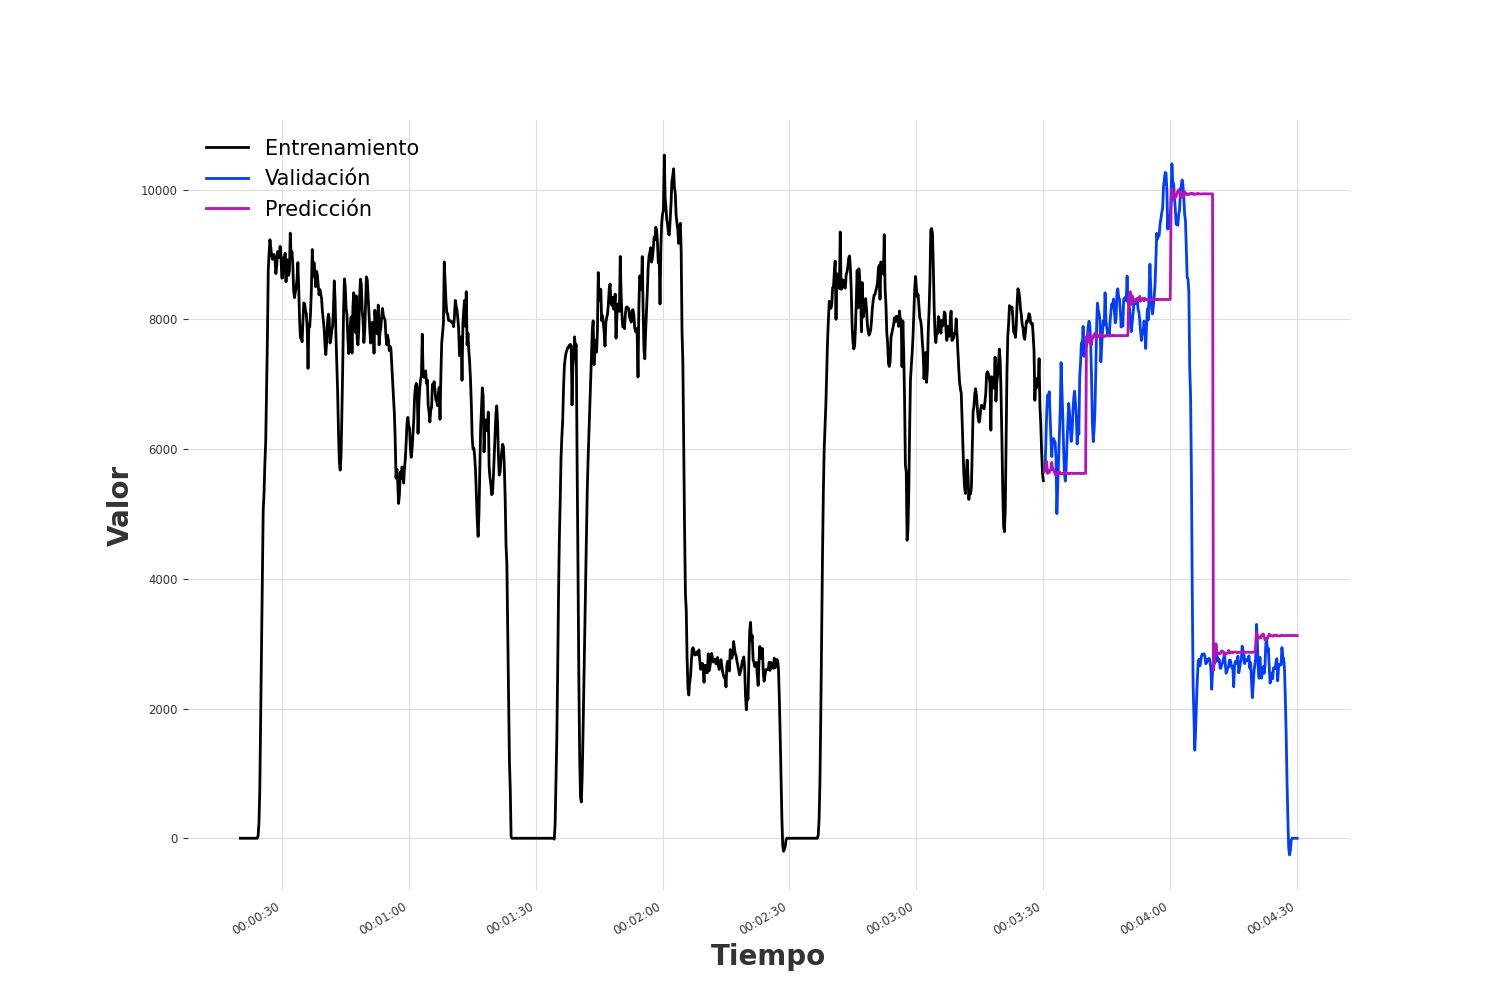
\includegraphics[width=1\textwidth,trim={1cm 0.7cm 1cm 2.5cm},clip]{arima_def}
    \caption{Predicción de ARIMA por defecto}\label{fig:arima_def}
\end{figure}

\begin{figure}[H]
    \centering
    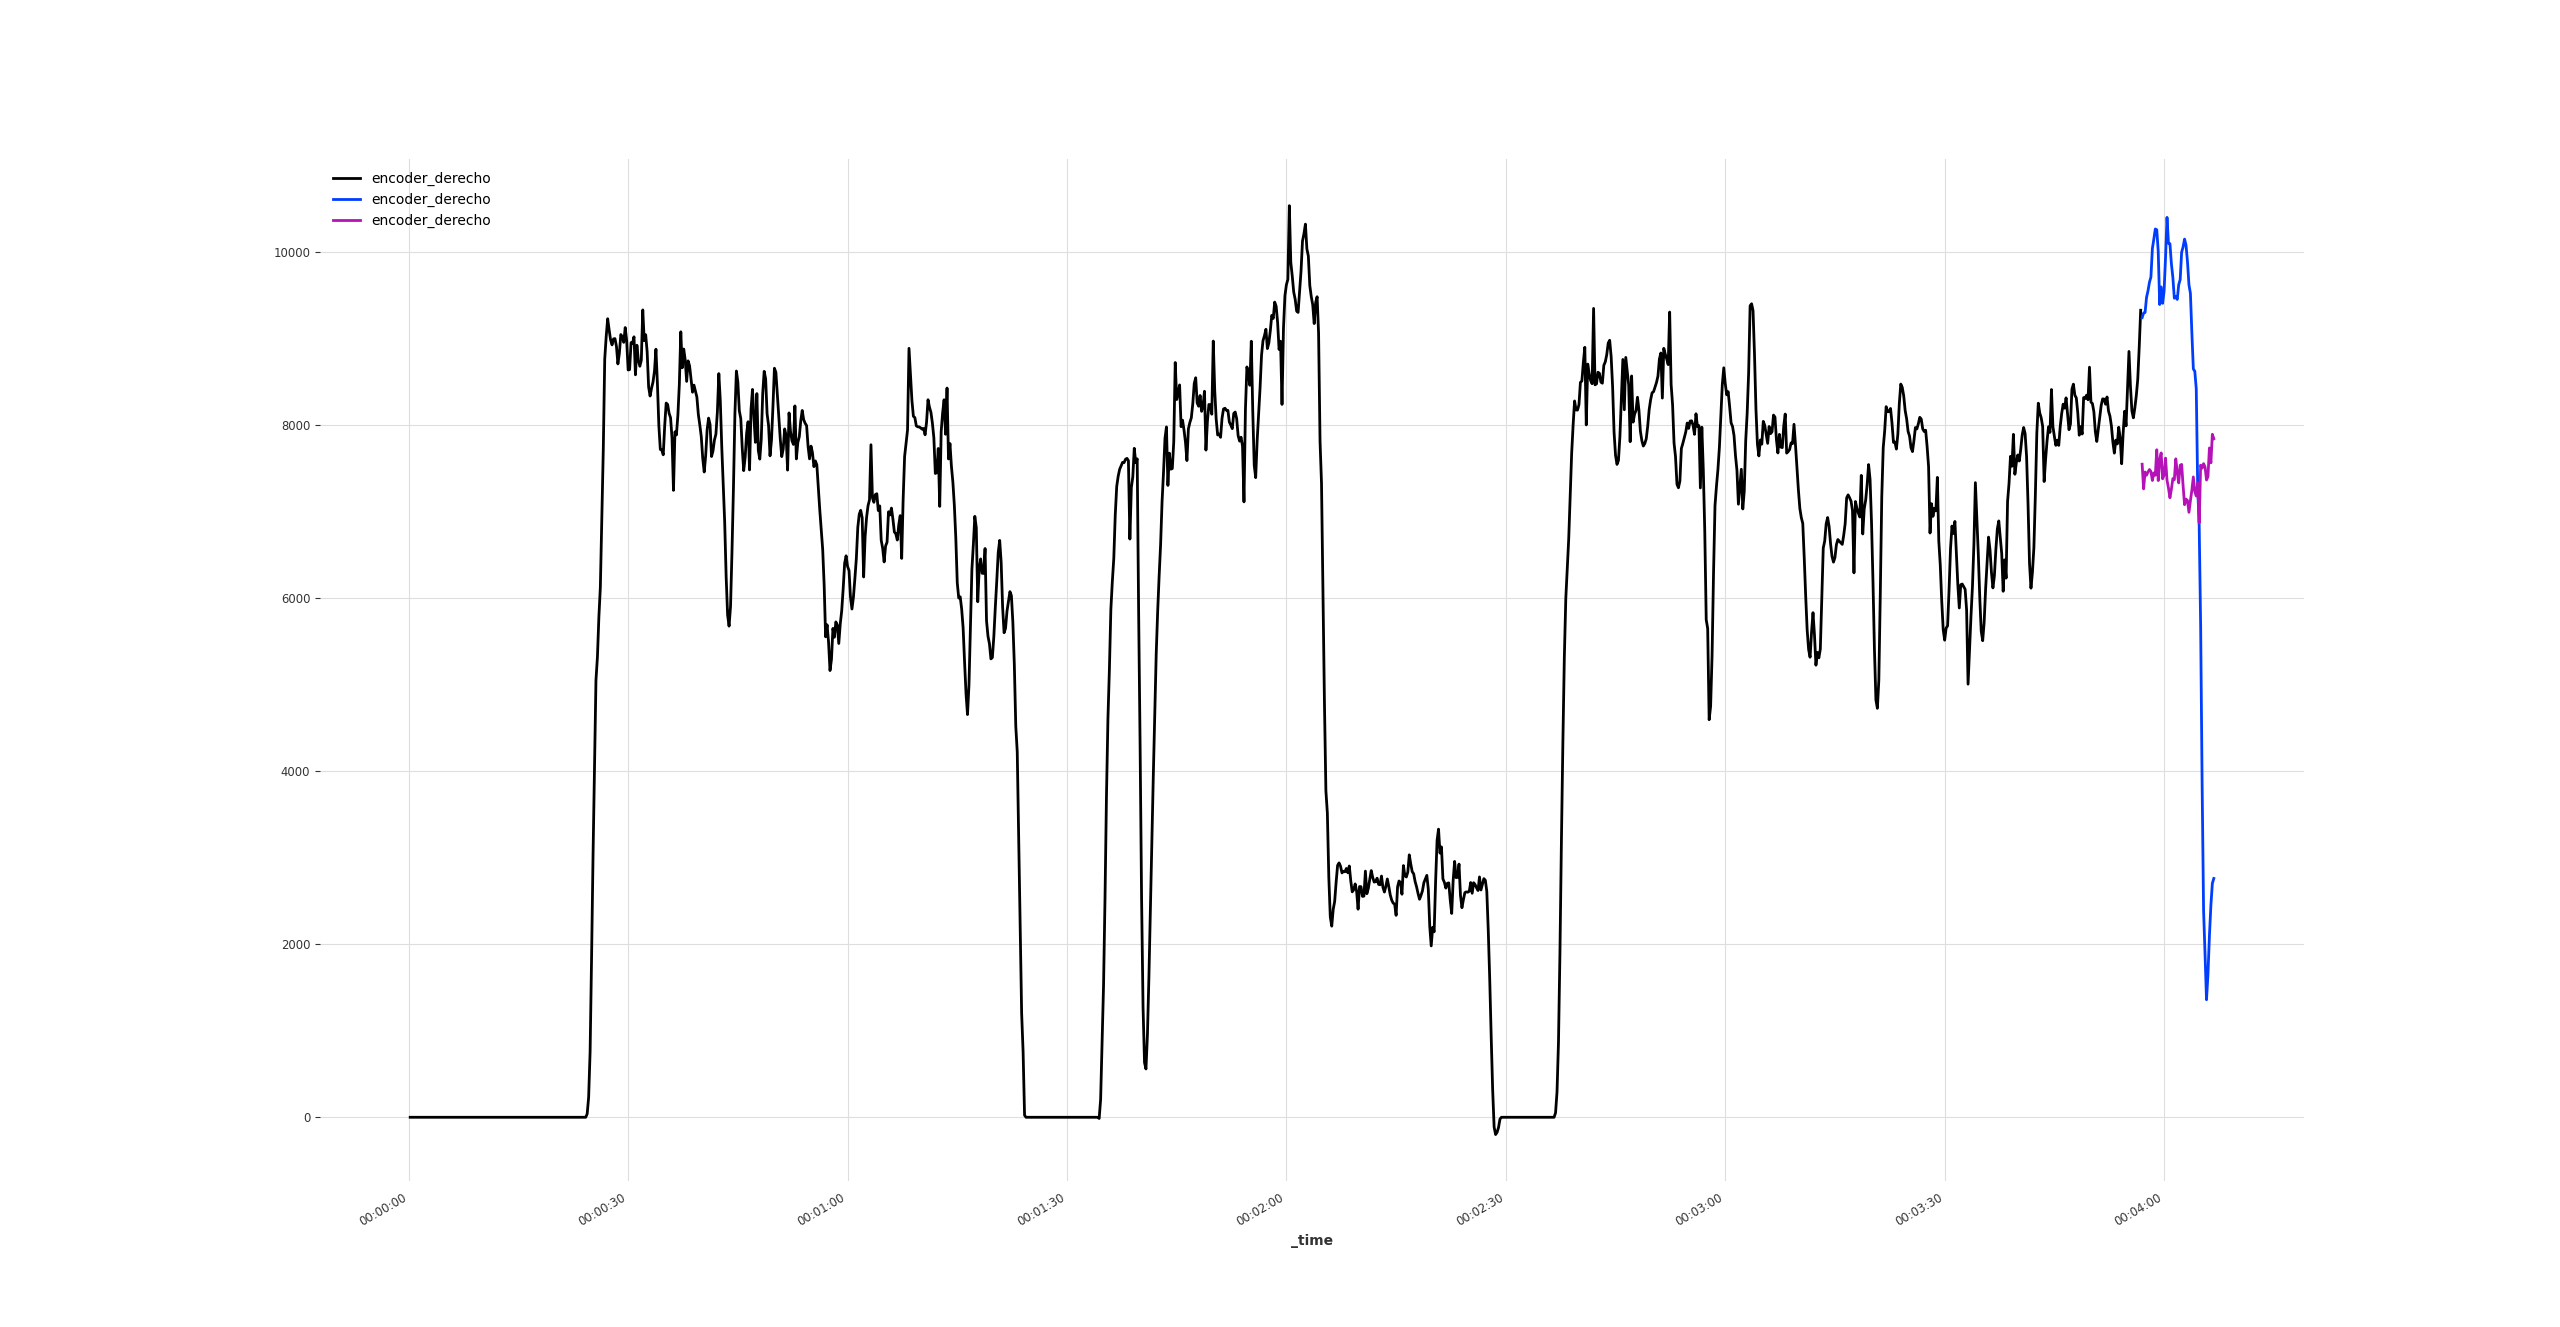
\includegraphics[width=1\textwidth,trim={1cm 0.7cm 1cm 2.5cm},clip]{tcn_def}
    \caption{Predicción de TCN por defecto}\label{fig:tcn_def}
\end{figure}

\begin{figure}[H]
    \centering
    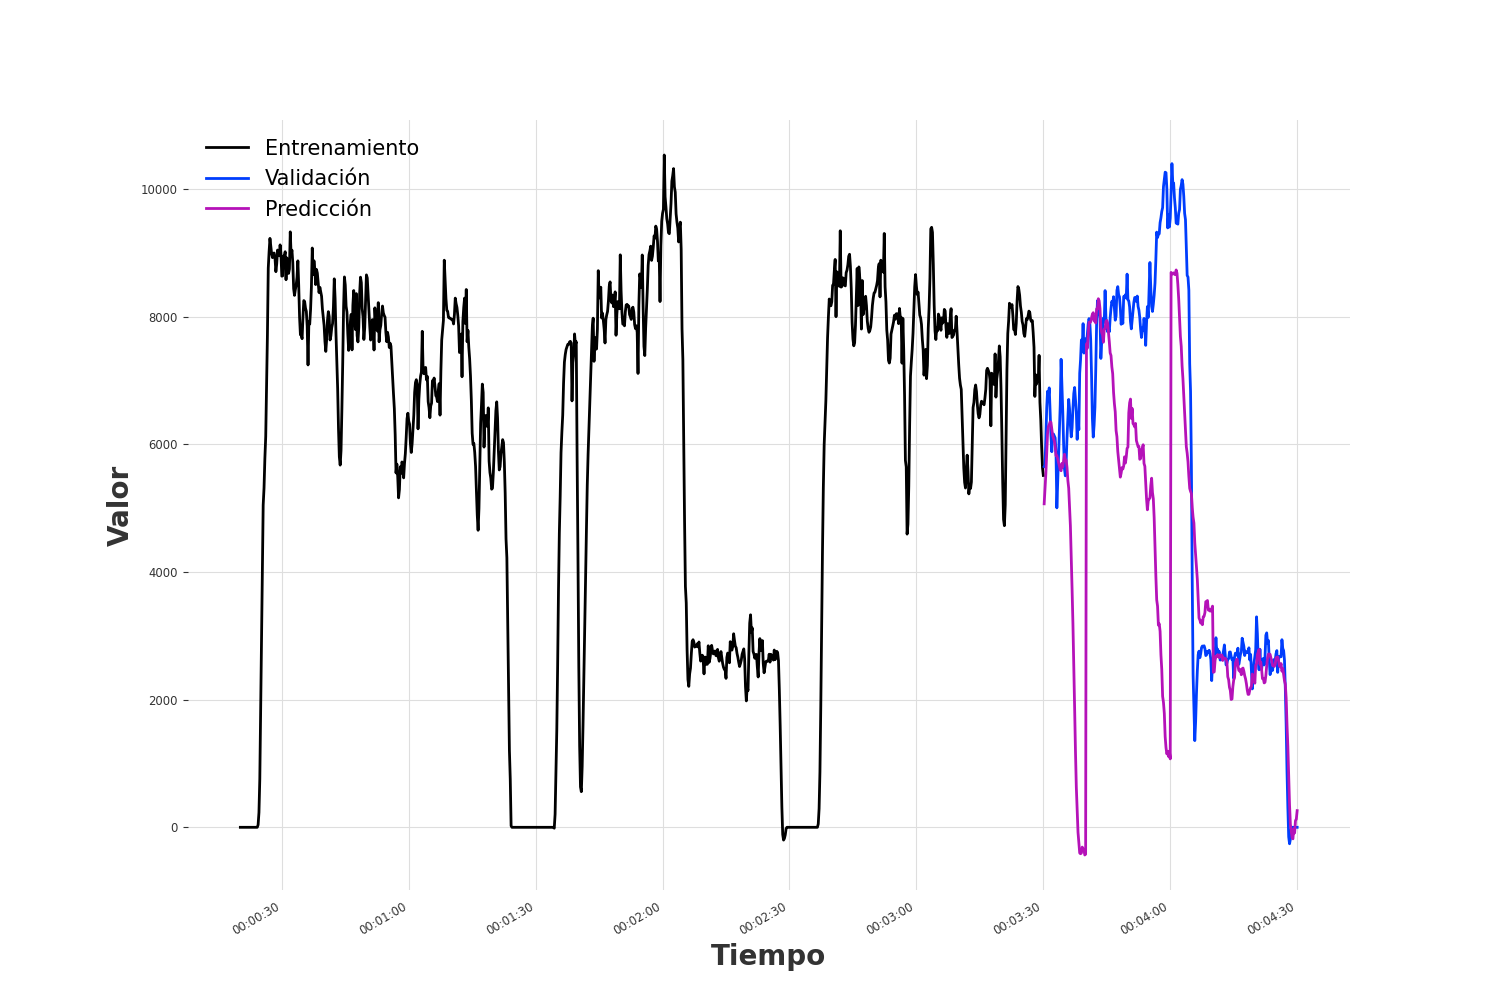
\includegraphics[width=1\textwidth,trim={1cm 0.7cm 1cm 2.5cm},clip]{nhits_def}
    \caption{Predicción de N-HiTS por defecto}\label{fig:nhits_def}
\end{figure}

\begin{figure}[H]
    \centering
    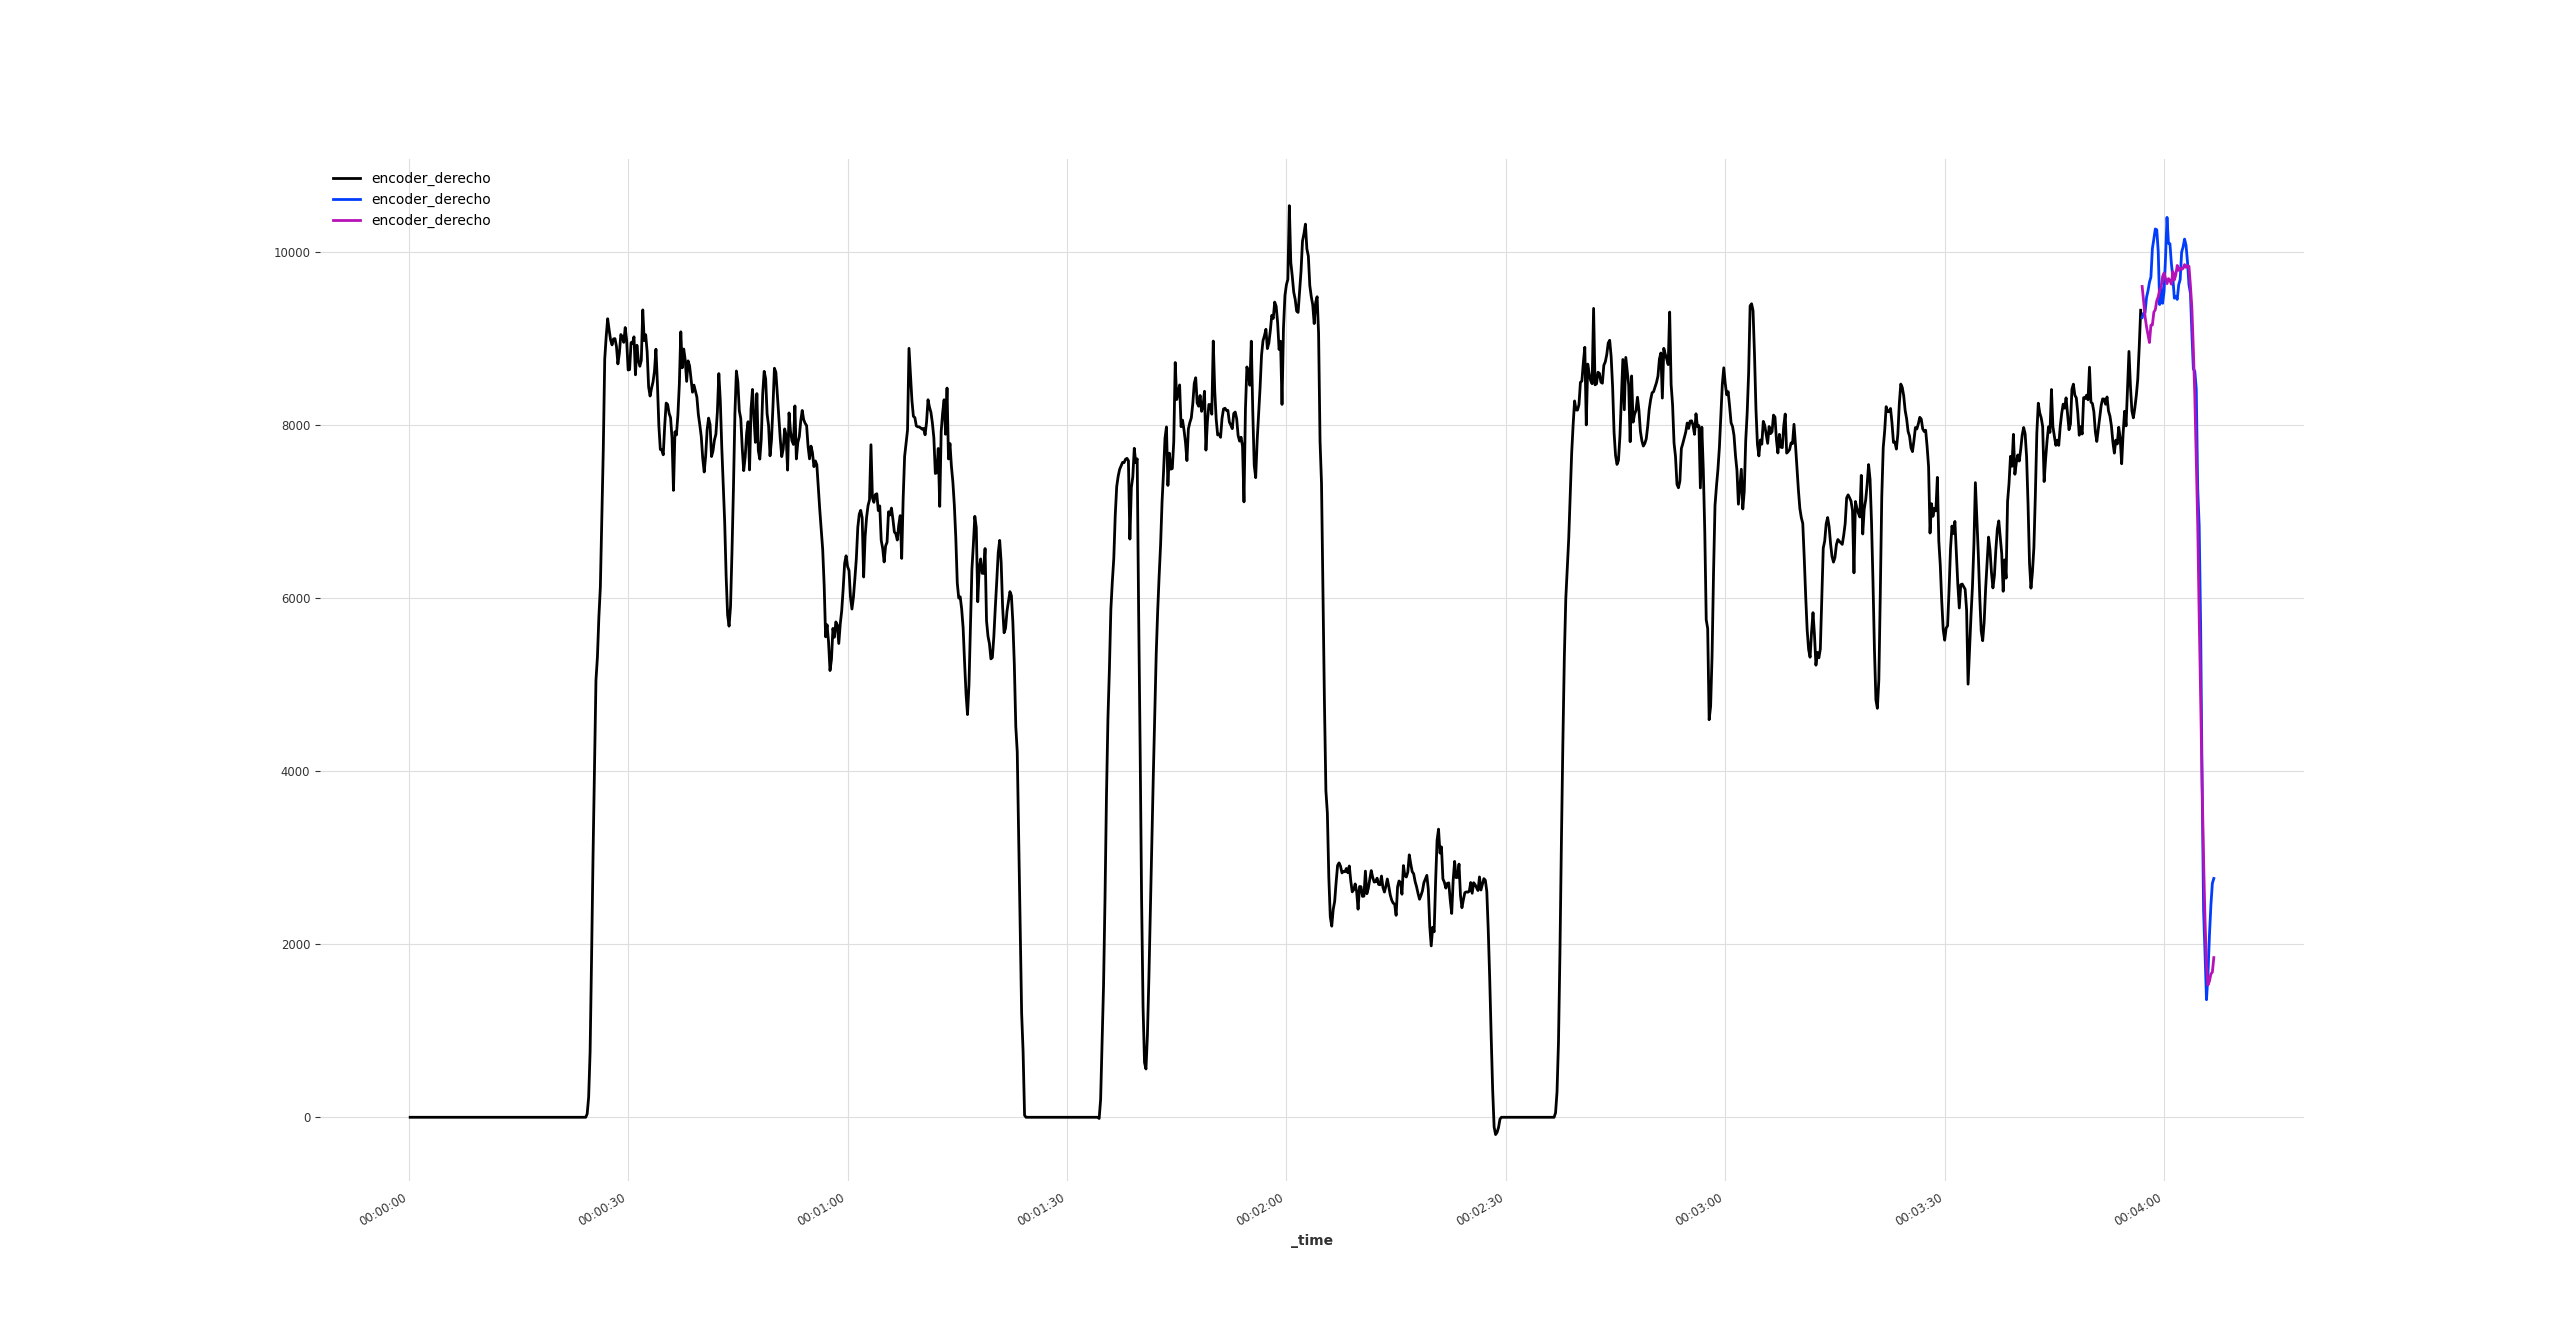
\includegraphics[width=1\textwidth,trim={1cm 0.7cm 1cm 2.5cm},clip]{transformer_def}
    \caption{Predicción de Transformer por defecto}\label{fig:transformer_def}
\end{figure}
% \imagenSized{arima_def}{}{0.8}
% \imagenSized{tcn_def}{}{0.8}
% \imagenSized{nhits_def}{}{0.8}
% \imagenSized{transformer_def}{}{0.8}

\subsection{Optimización de los hiperparámetros}

Los resultados del apartado anterior son potencialmente mejorables. Para ello, es necesario encontrar los parámetros de los 
modelos que mejor se ajusten a nuestros datos. Esto, sin embargo, no es una tarea simple, pues existe una enorme 
cantidad de ellos para los modelos que utilicen redes neuronales (TCN, N-HiTS y Transformer). Para la optimización 
de dichos modelos se ha utilizado una herramienta llamada Optuna. Esta herramienta prueba cada modelo durante 
varias horas probando diferentes combinaciones de hiperparámetros de manera automática.

Para el caso de ARIMA la optimización es más simple, pues, como se ha explicado en el apartado de conceptos 
teóricos solo tiene tres parámetros. Además, dichos parámetros pueden optimizarse de manera analítica, utilizando 
los gráficos de autocorrelación y autocorrelación parcial. El primero de estos muestra como de relacionado está 
un valor de la serie temporal con sus anteriores, mientras que el segundo muestra la correlación con el valor 
inmediatamente anterior al actual.

\imagenSized{acf}{ACF del encoder derecho}{1}
\imagenSized{pacf}{PACF del encoder derecho}{1}

Como podemos ver, el valor del ACF decrementa, pero de manera muy lenta, lo que nos indica que necesitamos 
por lo menos un orden de diferenciación, por lo que el parámetro d será por lo menos de 1. 

\imagenSized{acf_dif2}{ACF del encoder derecho después de diferenciar}{1}
\imagenSized{pacf_dif2}{PACF del encoder derecho después de diferenciar}{1}

Se puede ver también como a partir del elemento 16 no se aprecian valores significativos, por lo que el valor del 
parámetro p será 16. Estas observaciones nos indican a pensar que el modelo es ARIMA(p, d, 0), ya que se cumplen 
dichas condiciones:
\begin{itemize}
    \item El ACF decae de manera exponencial.
    \item En el PACF, hay un valor significativo a partir del valor p, pero ninguno más adelante.
\end{itemize}

Por todo esto, el modelo ARIMA que mejor se adapta a nuestro caso es ARIMA(16, 1, 0).

\subsection{Resultados tras la optimización}

Una vez optimizados los hiperparámetros de cada modelo, se vuelve a realizar la comparación.

\begin{table}[H]
    \centering
    \begin{adjustbox}{max width=\textwidth}
        \begin{tabular}{c | c c c | c c c | c c c}
            \toprule
            & \multicolumn{3}{c | }{Univariante} & \multicolumn{3}{c | }{Covariante} & \multicolumn{3}{c}{Multivariante} \\
            Tiempo & 0.2 & 1 & 10 & 0.2 & 1 & 10 & 0.2 & 1 & 10 \\
            \otoprule
            ARIMA & \textbf{156.587} & 402.922 & 1222.479 & - & - & - & - & - & - \\
            TCN & 1584.048 & 1611.392 & 1898.327 & 1568.804 & 1596.126 & 1631.922 & 1256.715 & 1974.812 & 1787.258 \\
            N-HiTS & 313.865 & 642.887 & 1429.619 & 349.071 & \textbf{396.670} & 1140.826 & 413.604 & 495.936 & \textbf{973.573} \\
            Transformer & 312.591 & 442.846 & 1292.514 & 450.393 & 410.858 & 1119.789 & 683.099 & 604.807 & 1062.630 \\
            \bottomrule
        \end{tabular}
    \end{adjustbox}
    \caption{MAE de los modelos optimizados}
    \label{tab:mae_opt}
\end{table}

\begin{table}[H]
    \centering
    \begin{adjustbox}{max width=\textwidth}
        \begin{tabular}{c | c c c | c c c | c c c}
            \toprule
            & \multicolumn{3}{c | }{Univariante} & \multicolumn{3}{c | }{Covariante} & \multicolumn{3}{c}{Multivariante} \\
            Tiempo & 0.2 & 1 & 10 & 0.2 & 1 & 10 & 0.2 & 1 & 10 \\
            \otoprule
            ARIMA & \textbf{0.665} & 1.713 & 5.206 & - & - & - & - & - & - \\
            TCN & 6.708 & 6.824 & 8.032 & 6.628 & 6.751 & 6.904 & 5.335 & 8.345 & 7.553 \\
            N-HiTS & 1.331 & 2.724 & 6.047 & 1.483 & \textbf{1.688} & 4.828 & 1.753 & 2.106 & \textbf{4.126} \\
            Transformer & 1.329 & 1.882 & 5.490 & 1.910 & 1.748 & 4.746 & 2.907 & 2.573 & 4.488 \\
            \bottomrule
        \end{tabular}
    \end{adjustbox}    
    \caption{MASE de los modelos optimizados}
    \label{tab:mase_opt}
\end{table}

\begin{table}[H]
    \centering
    \begin{adjustbox}{max width=\textwidth}
        \begin{tabular}{c | c c c | c c c | c c c}
            \toprule
            & \multicolumn{3}{c | }{Univariante} & \multicolumn{3}{c | }{Covariante} & \multicolumn{3}{c}{Multivariante} \\
            Tiempo & 0.2 & 1 & 10 & 0.2 & 1 & 10 & 0.2 & 1 & 10 \\
            \otoprule
            ARIMA & \textbf{156.587} & \textbf{371.751} & 1059.898 & - & - & - & - & - & - \\
            TCN & 1584.048 & 1587.879 & 1218.422 & 1568.804 & 1574.762 & 650.782 & 1256.715 & 1950.265 & 910.187 \\
            N-HiTS & 313.865 & 629.109 & 973.335 & 349.071 & 375.828 & 692.528 & 413.604 & 460.923 & 545.182 \\
            Transformer & 312.591 & 393.569 & 723.987 & 450.393 & 358.407 & \textbf{515.197} & 683.099 & 554.948 & 707.391 \\
            \bottomrule
        \end{tabular}
    \end{adjustbox}
    \caption{DTW de los modelos optimizados}
    \label{tab:dtw_opt}
\end{table}

\begin{table}[H]
    \centering
    \begin{adjustbox}{max width=\textwidth}
        \begin{tabular}{c | c c c | c c c | c c c}
            \toprule
            & \multicolumn{3}{c | }{Univariante} & \multicolumn{3}{c | }{Covariante} & \multicolumn{3}{c}{Multivariante} \\
            Tiempo & 0.2 & 1 & 10 & 0.2 & 1 & 10 & 0.2 & 1 & 10 \\
            \otoprule
            ARIMA & \textbf{0.875} & \textbf{0.823} & \textbf{0.687} & - & - & - & - & - & - \\
            TCN & 36.238 & 37.601 & 35.455 & 42.710 & 42.582 & 42.831 & 35.664 & 33.898 & 34.281 \\
            N-HiTS & 92.157 & 96.569 & 92.305 & 100.803 & 99.655 & 101.466 & 93.489 & 90.949 & 92.417 \\
            Transformer & 101.097 & 100.450 & 107.295 & 108.456 & 109.764 & 114.103 & 104.710 & 101.225 & 110.707 \\
            \bottomrule
        \end{tabular}
    \end{adjustbox}
    \caption{Tiempo de ajuste en segundos de los modelos optimizados}
    \label{tab:te_opt}
\end{table}

\begin{table}[H]
    \centering
    \begin{adjustbox}{max width=\textwidth}
        \begin{tabular}{c | c c c | c c c | c c c}
            \toprule
            & \multicolumn{3}{c | }{Univariante} & \multicolumn{3}{c | }{Covariante} & \multicolumn{3}{c}{Multivariante} \\
            Tiempo & 0.2 & 1 & 10 & 0.2 & 1 & 10 & 0.2 & 1 & 10 \\
            \otoprule
            ARIMA & 0.052 & 0.049 & 0.048 & - & - & - & - & - & - \\
            TCN & 0.021 & 0.016 & 0.015 & \textbf{0.019} & \textbf{0.014} & \textbf{0.015} & 0.019 & 0.015 & 0.016 \\
            N-HiTS & 0.025 & 0.028 & 0.025 & 0.025 & 0.027 & 0.025 & 0.027 & 0.025 & 0.026 \\
            Transformer & 0.027 & 0.025 & 0.025 & 0.025 & 0.029 & 0.026 & 0.026 & 0.027 & 0.029 \\
            \bottomrule
        \end{tabular}
    \end{adjustbox}
    \caption{Tiempo de predicción en segundos de los modelos optimizados}
    \label{tab:tp_opt}
\end{table}

A continuación se ven los resultados de las predicciones realizadas con los modelos optimizados. 
Al igual que en la anterior prueba, se predicen los próximos 10 segundos utilizando covariables 
(excepto en el caso de ARIMA que no lo soporta). En negro se ven los valores pasados, en morado 
los valores predichos y en azul los valores reales para comparar.

\begin{figure}[H]
    \centering
    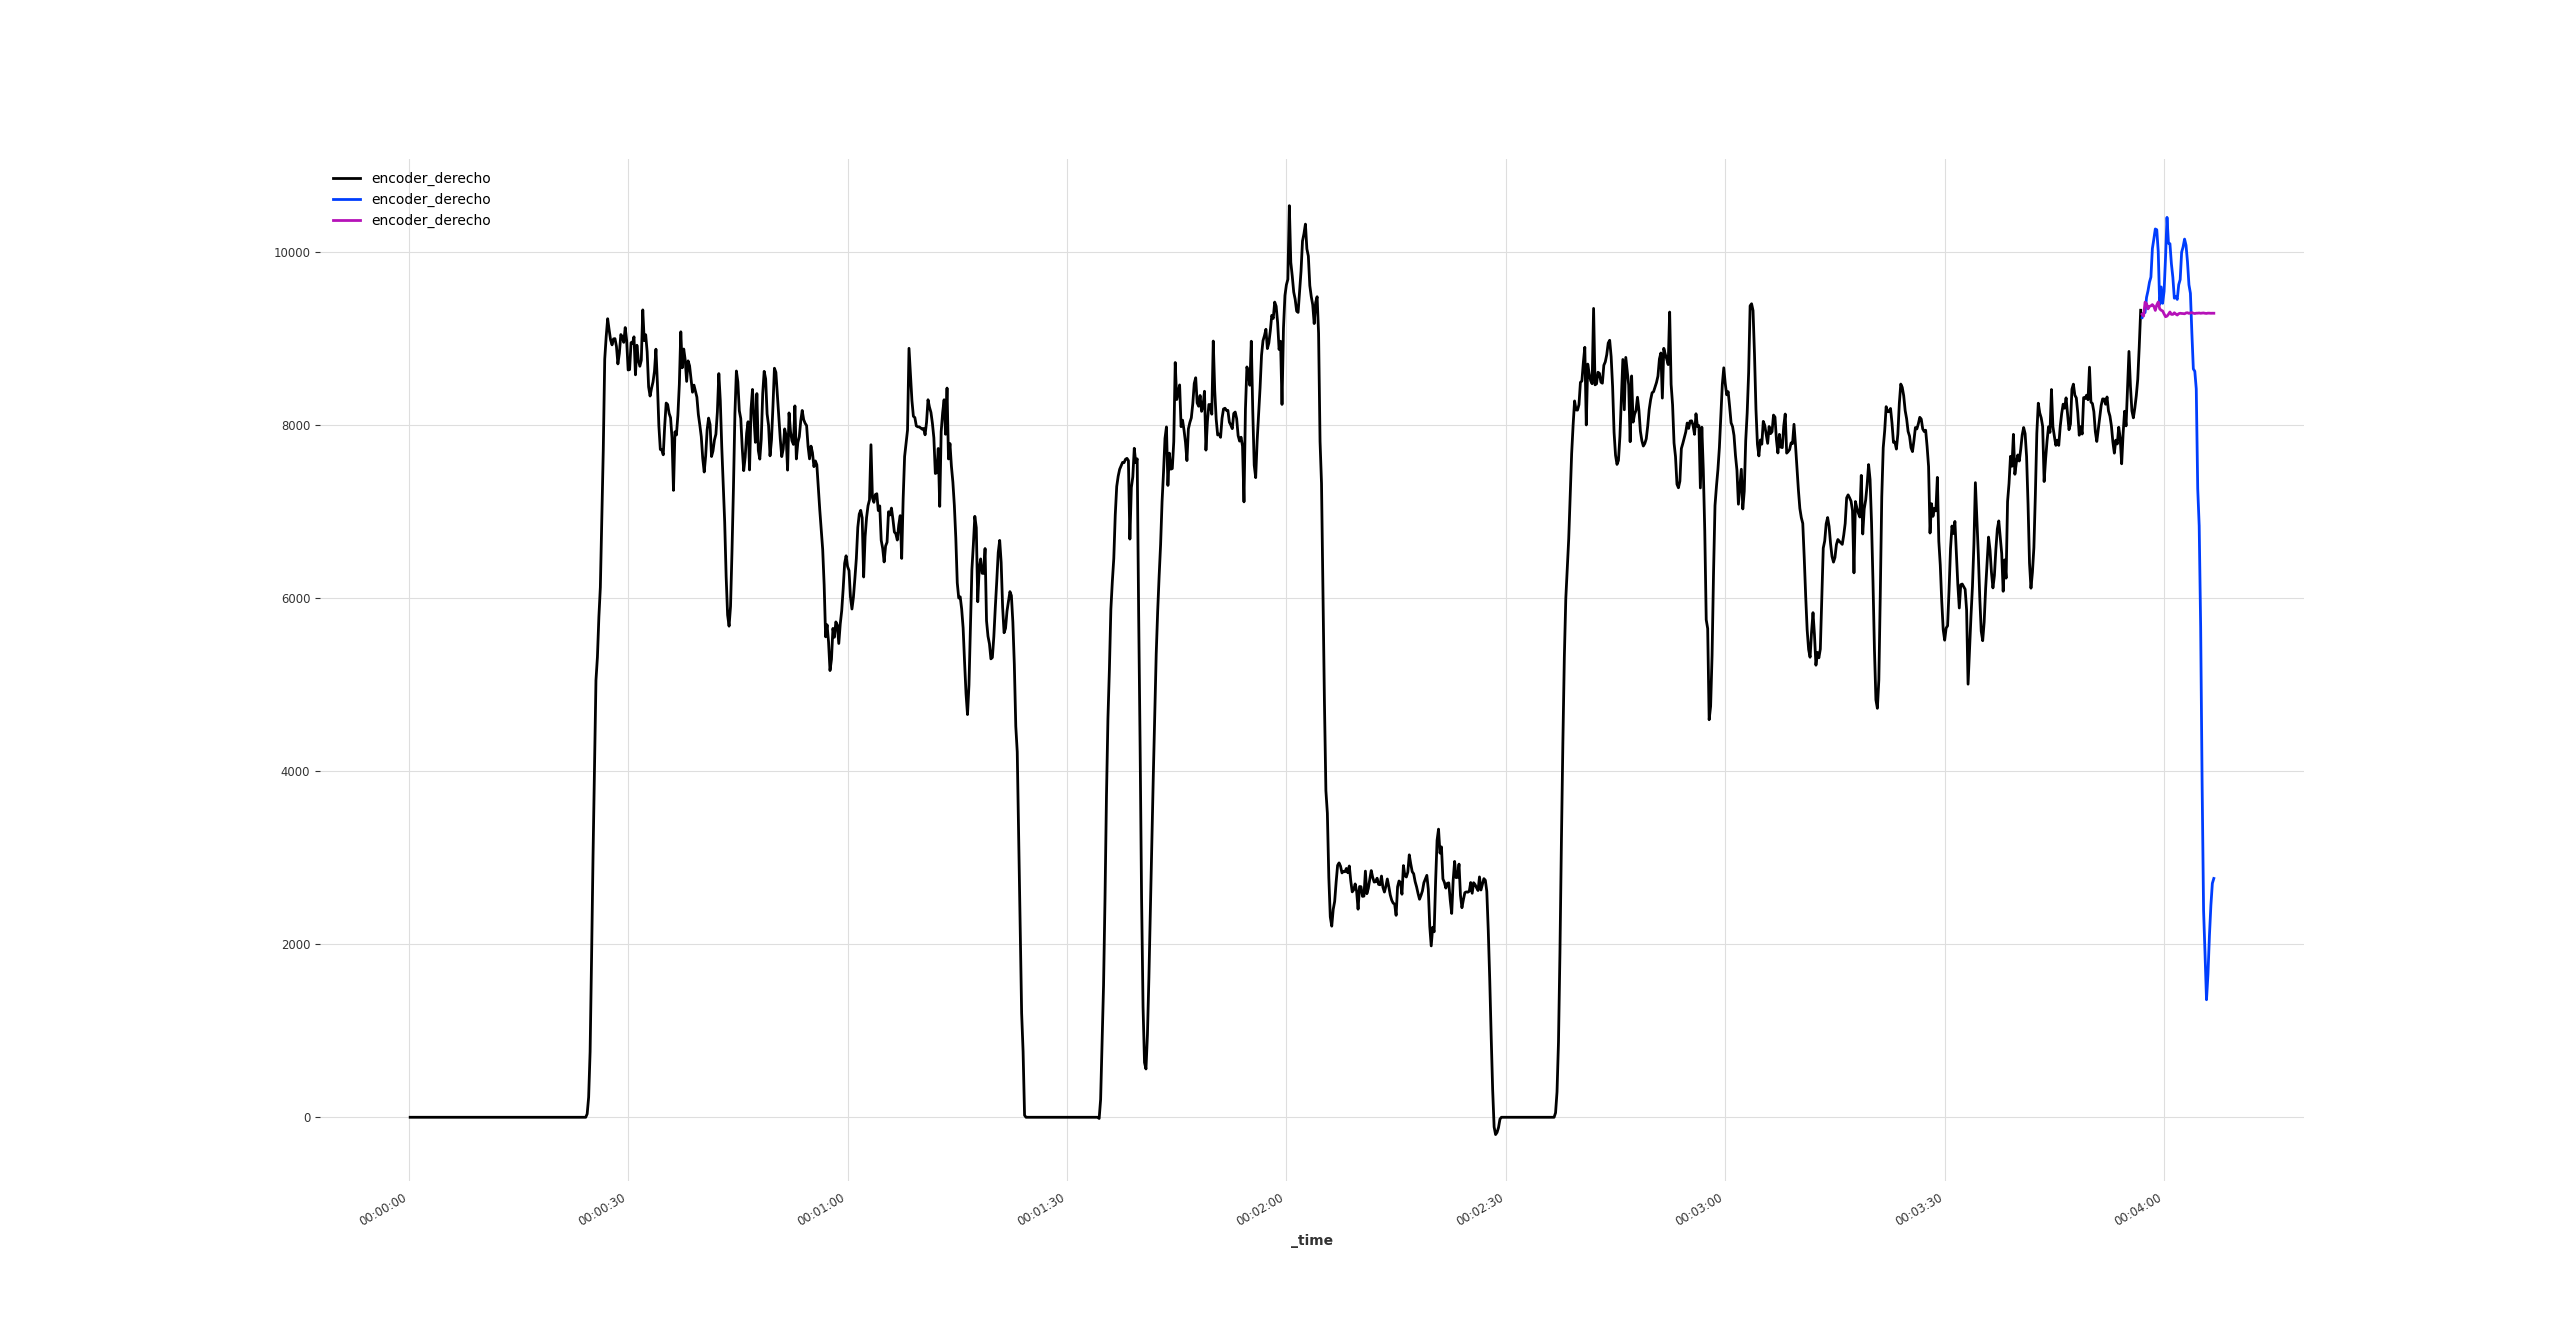
\includegraphics[width=1\textwidth,trim={1cm 0.7cm 1cm 2.5cm},clip]{arima_opt}
    \caption{Predicción de ARIMA con optimización}\label{fig:arima_opt}
\end{figure}

\begin{figure}[H]
    \centering
    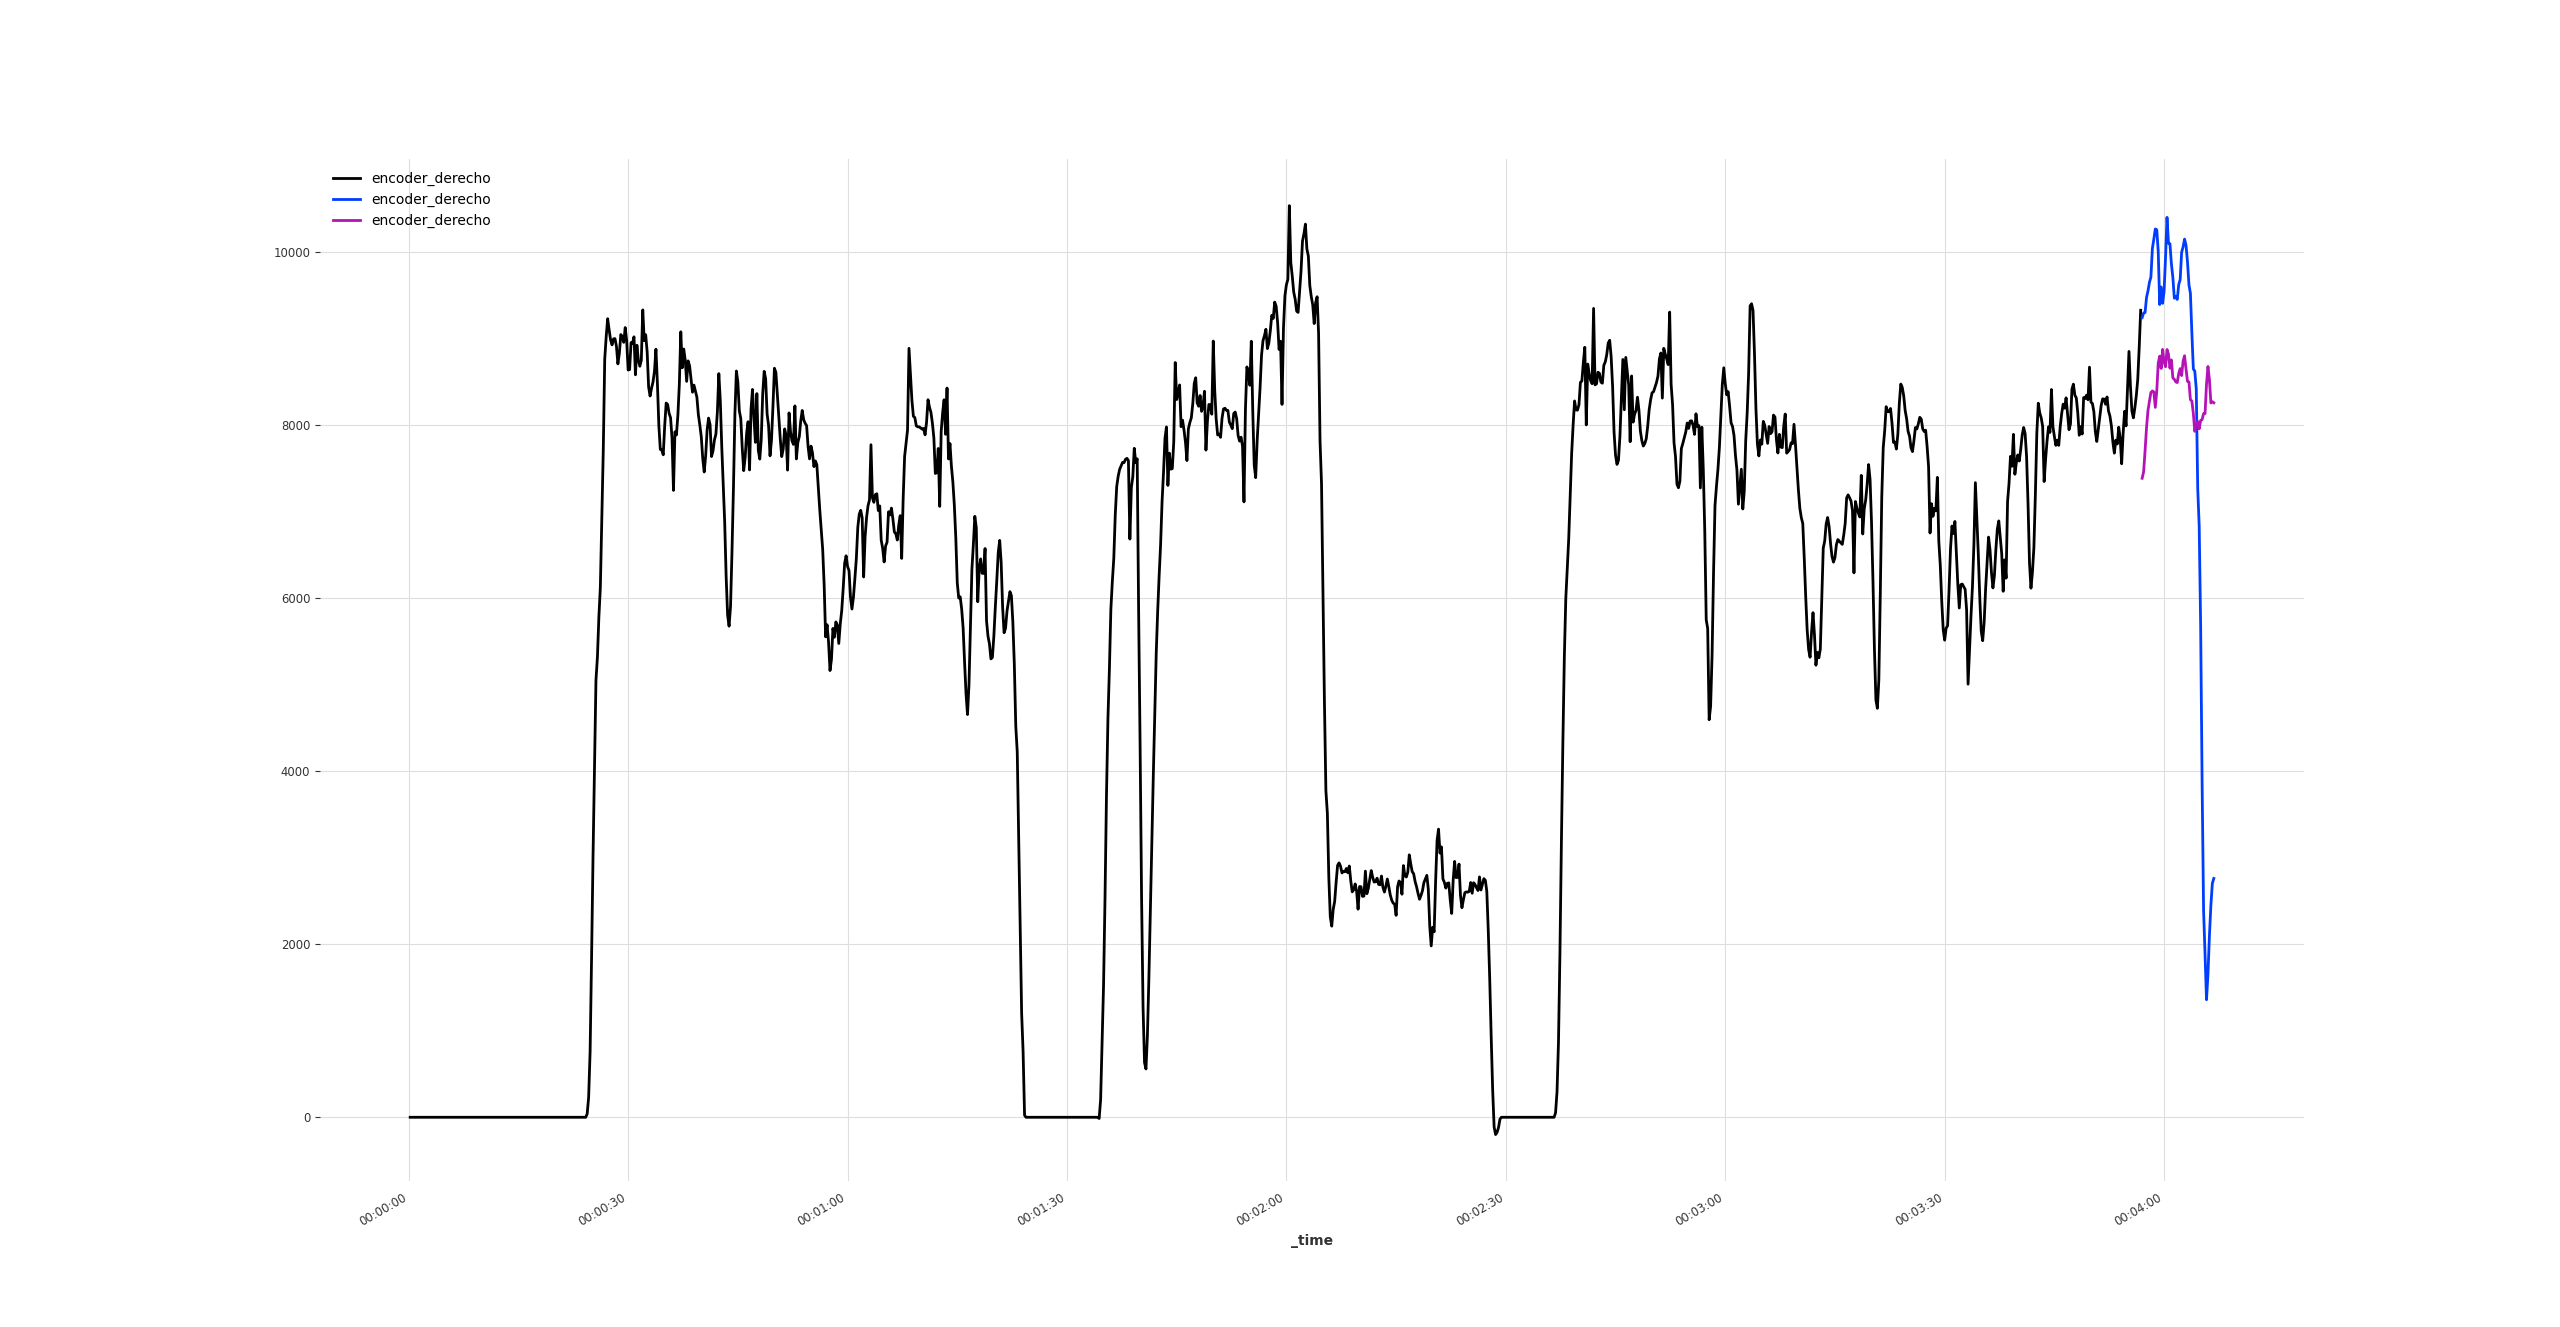
\includegraphics[width=1\textwidth,trim={1cm 0.7cm 1cm 2.5cm},clip]{tcn_opt}
    \caption{Predicción de TCN con optimización}\label{fig:tcn_opt}
\end{figure}

\begin{figure}[H]
    \centering
    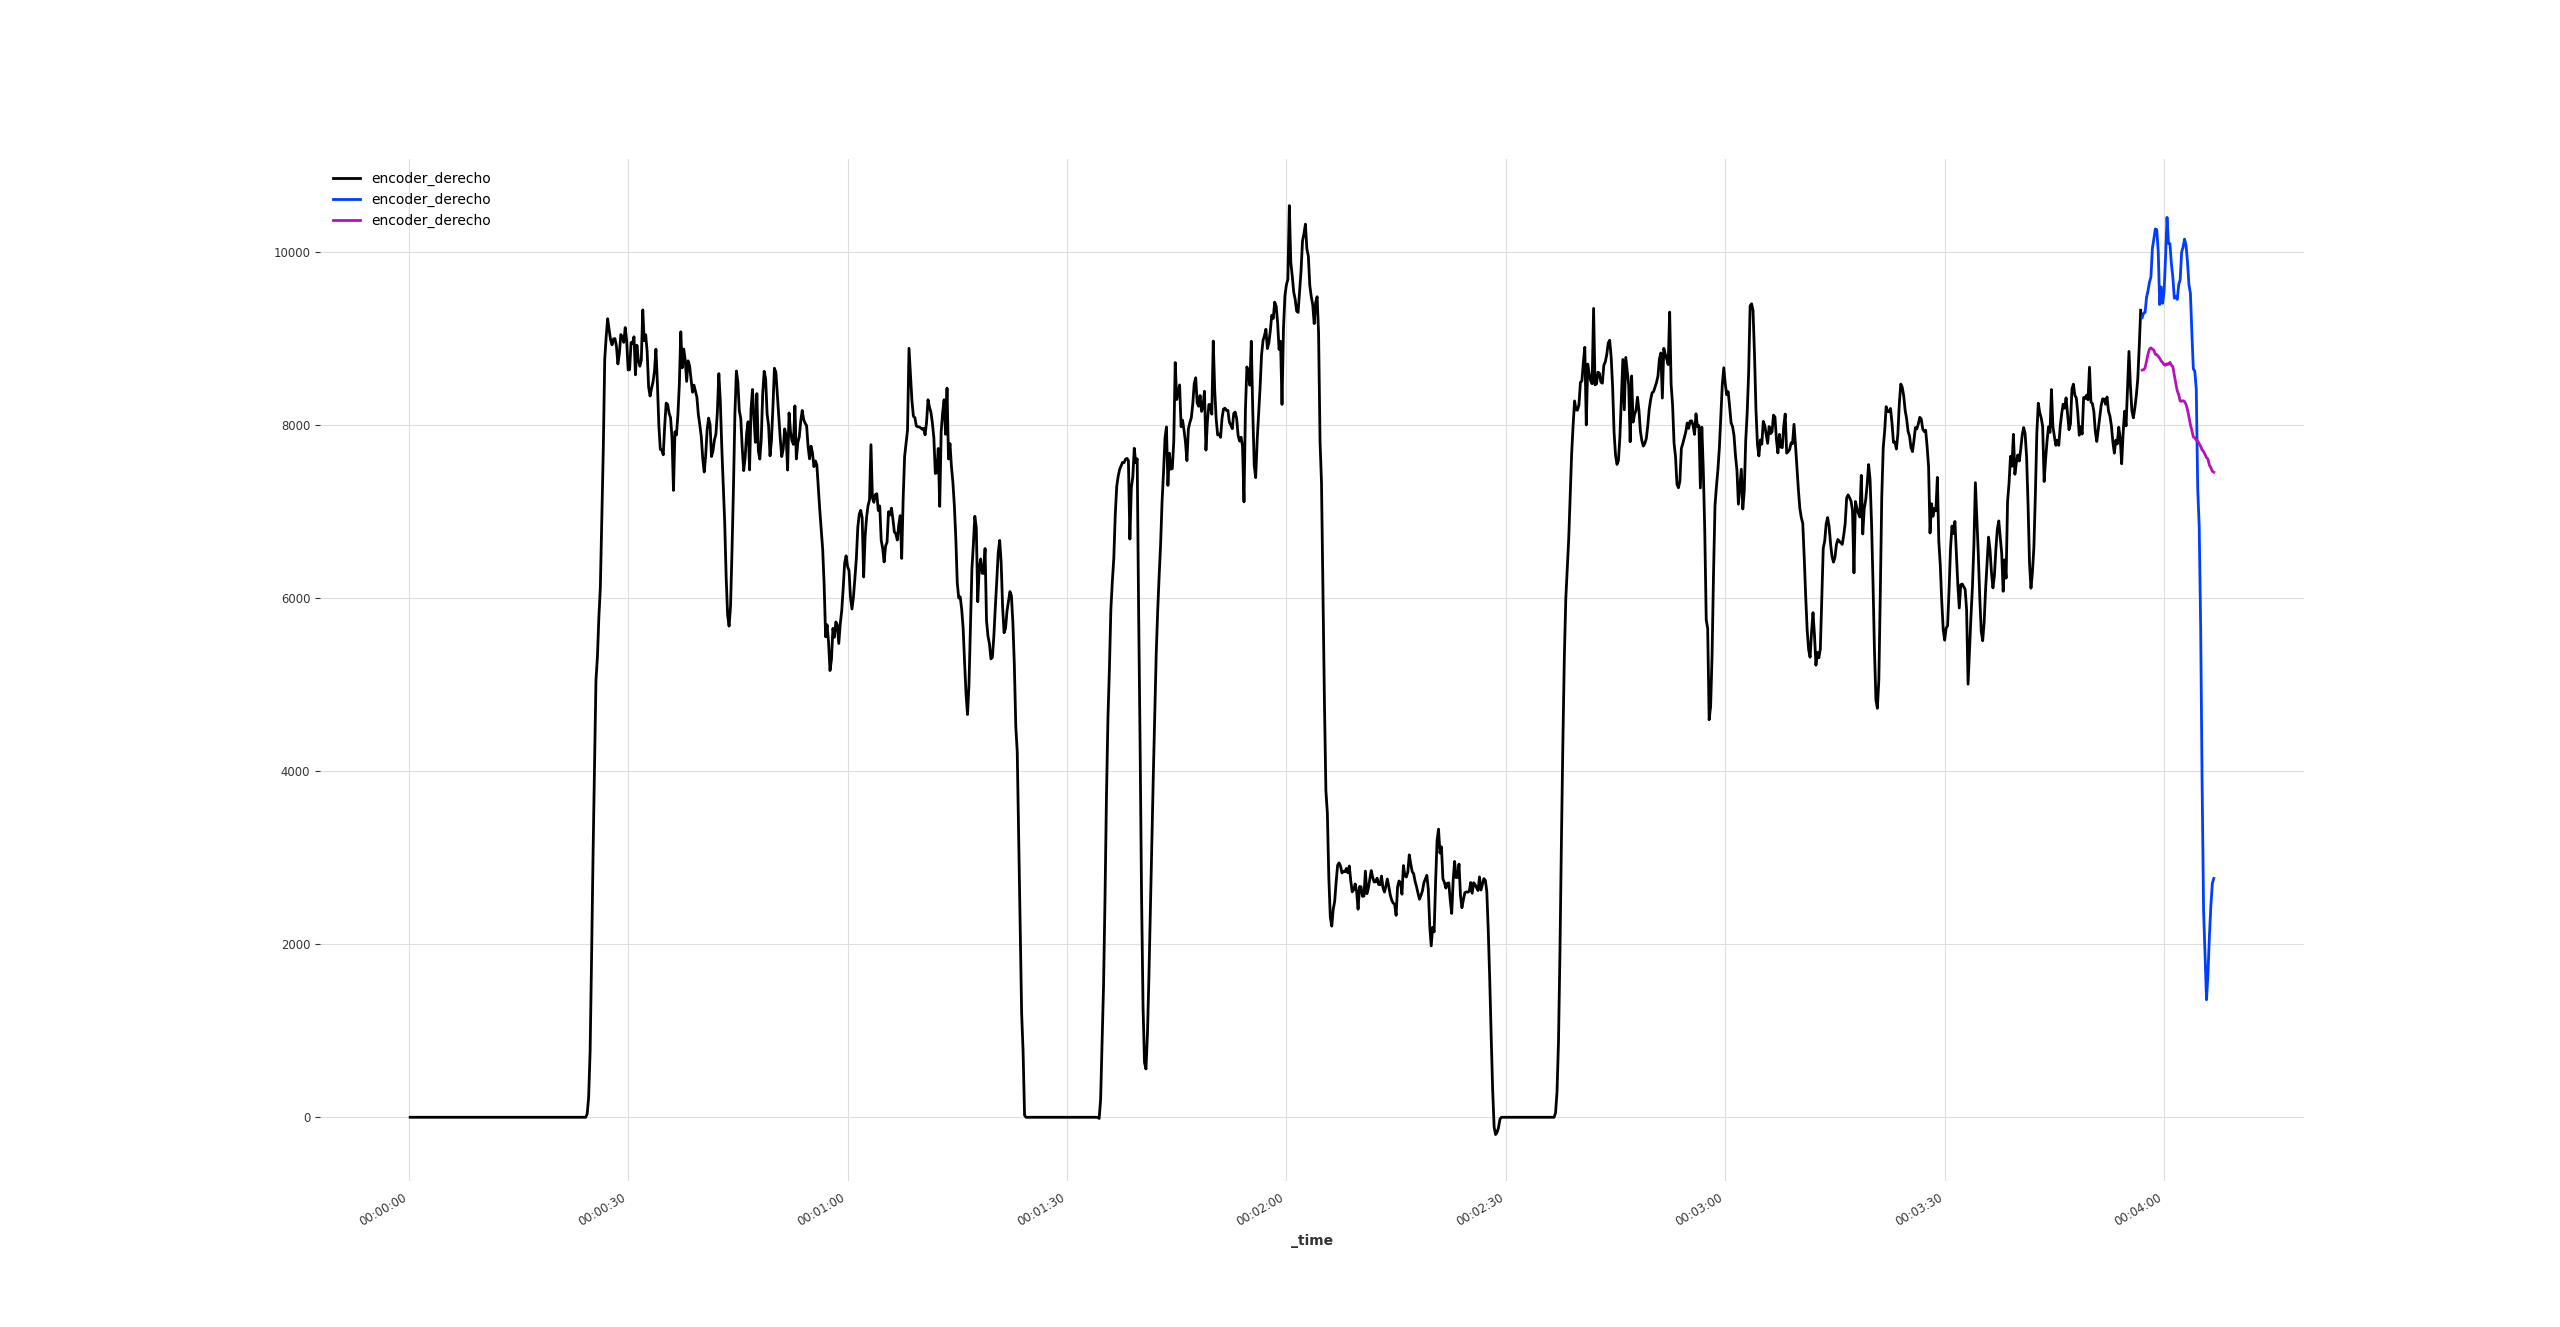
\includegraphics[width=1\textwidth,trim={1cm 0.7cm 1cm 2.5cm},clip]{nhits_opt}
    \caption{Predicción de N-HiTS con optimización}\label{fig:nhits_opt}
\end{figure}

\begin{figure}[H]
    \centering
    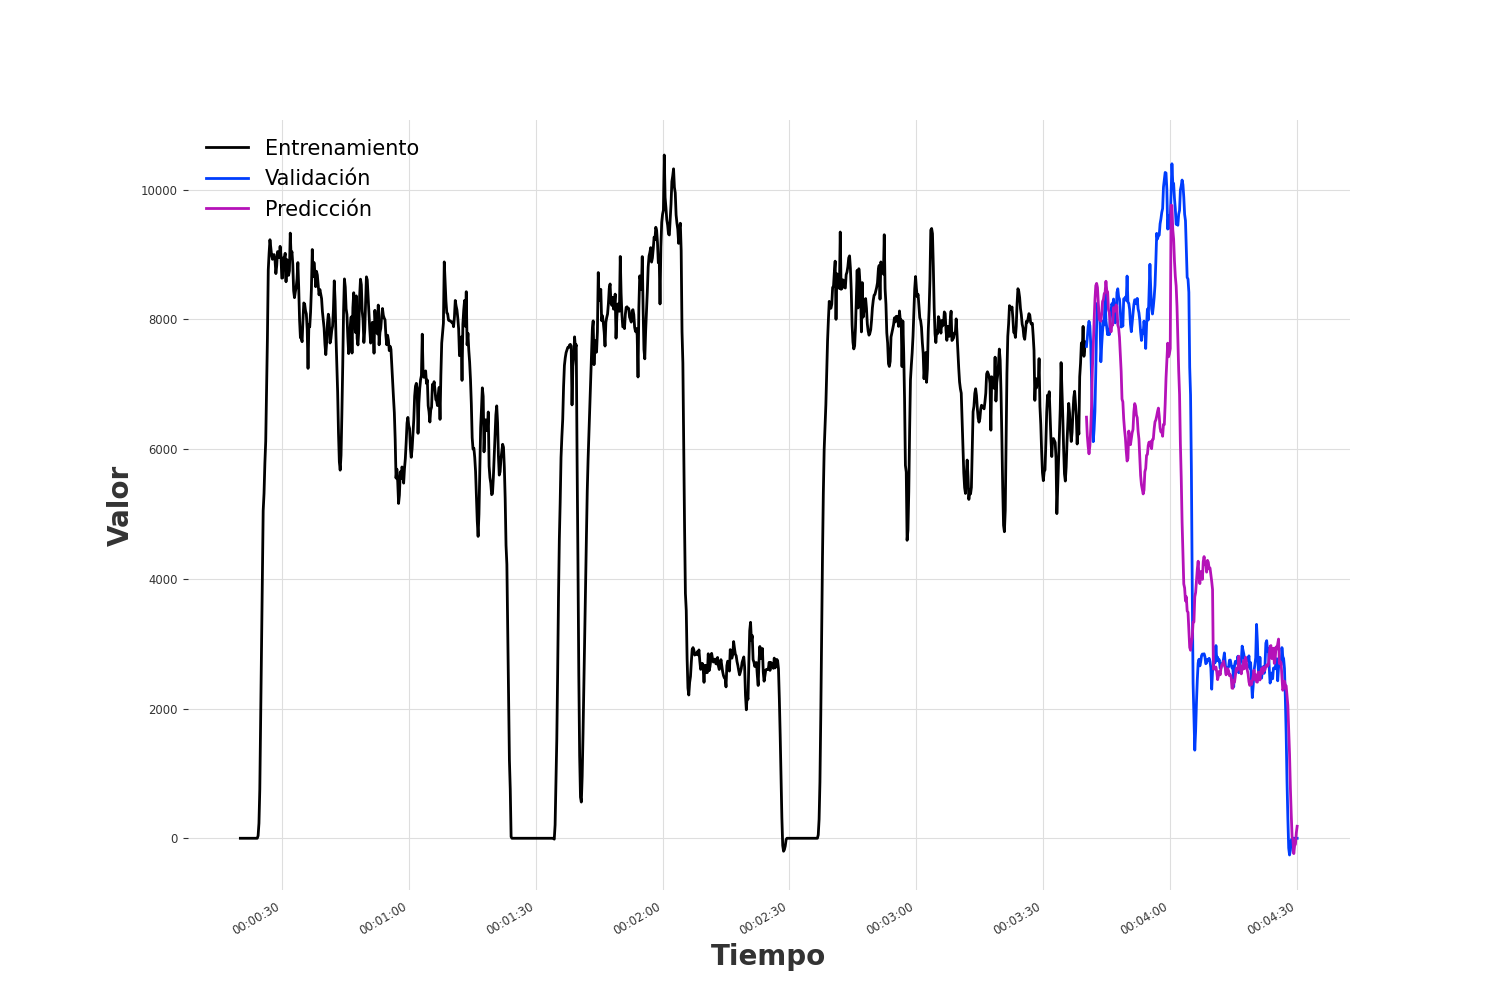
\includegraphics[width=1\textwidth,trim={1cm 0.7cm 1cm 2.5cm},clip]{transformer_opt}
    \caption{Predicción de Transformer con optimización}\label{fig:transformer_opt}
\end{figure}

% \imagenSized{arima_opt}{Predicción de ARIMA con optimización}{0.8}
% \imagenSized{tcn_opt}{Predicción de TCN con optimización}{0.8}
% \imagenSized{nhits_opt}{Predicción de N-HiTS con optimización}{0.8}
% \imagenSized{transformer_opt}{Predicción de Transformer con optimización}{0.8}

\subsection{Conclusiones}

% Como se puede observar, excepto en ARIMA, la optimización arroja peores resultados que los modelos por defecto. Esto 
% se puede deber principalmente a tres factores:
% \begin{enumerate}
%     \item Los modelos por defecto son lo suficientemente buenos.
%     \item El tiempo de ejecución de la optimización no ha sido el suficiente, por lo que no se han encontrado las 
%         mejores combinaciones de hiperparámetros.
%     \item La cantidad de datos utilizada para el entrenamiento no es suficiente.
% \end{enumerate}

% En cuanto a ARIMA, a cambio de obtener mejores resultados tanto el tiempo de entrenamiento como el de predicción 
% son algo más del doble de grandes. Tampoco supone un gran problema, ya que a la hora de entrenar solo 
% supone unos segundos más, y en el caso de la predicción el aumento está en el rango de los milisegundos.

Como se puede ver, la optimización ha mejorado la mayoría de resultados, a costa de aumentar el tiempo de
ajuste y el de predicción. Se sacan por tanto las siguientes conclusiones de las siguientes tablas y figuras:
\begin{enumerate}
    % \item El modelo transformador no mejora especialmente con la optimización, en especial en predicciones
    %     a 10 segundos en el futuro, que es el rango de tiempo que queremos predecir. El resto de modelos 
    %     mejoran ligeramente en la mayoría de casos.
    \item Los mejores modelos en predicciones a 10 segundos en el futuro son el transformador por defecto y 
        con covariables, o N-HiTS con optimizado con multivariables. Ya que trabajar en Darts con covariables 
        es más simple que con multivariables, se escogerá el primero.
    \item La cantidad de datos utilizada para el entrenamiento no es suficiente. Se habrían podido conseguir mejores
        resultados con un conjunto de datos más grande.
    \item El tiempo de optimización en el caso del modelo transformador no ha sido suficiente.
\end{enumerate}

Por todo esto, como queremos realizar predicciones a relativamente largo plazo (10 segundos), el modelo escogido 
finalmente será el Transformer con los hiperparámetros por defecto y con covariables. Aunque existen casos en los que 
este modelo no es el mejor, tiene un buen balance entre los tiempos de ajuste y predicción y resultados en el resto 
de métricas.

En el caso de que en un futuro quieran integrarse estas predicciones en el propio software del AGV con el fin 
de mejorar su rendimiento, habría que estudiar si usar ARIMA por sus buenos resultados a corto plazo, aunque habría 
que comprobar que los tiempos de predicción sean lo suficientemente buenos.